%% This is repurposed from `sample-sigconf.tex'
\documentclass[sigconf,review,authordraft]{acmart}


\usepackage{graphicx}
\usepackage{hyperref}
\usepackage{cleveref}
\usepackage{tabulary}
\usepackage{soul}
\usepackage{subcaption}
\usepackage{algorithm}
\usepackage{algorithmic}

% pseudocode cpp
\usepackage{listings}
\usepackage{xcolor}


%%
%% \BibTeX command to typeset BibTeX logo in the docs
\AtBeginDocument{%
  \providecommand\BibTeX{{%
    \normalfont B\kern-0.5em{\scshape i\kern-0.25em b}\kern-0.8em\TeX}}}

%% Rights management information.  This information is sent to you
%% when you complete the rights form.  These commands have SAMPLE
%% values in them; it is your responsibility as an author to replace
%% the commands and values with those provided to you when you
%% complete the rights form.
%\setcopyright{acmcopyright}
%\copyrightyear{2018}
%\acmYear{2018}
%\acmDOI{10.1145/1122445.1122456}

%% These commands are for a PROCEEDINGS abstract or paper.
\acmConference[Under review for The Web Conference 2021]{The Web Conference 2021}{April 19--23, 2021}{Ljubljana, Slovenia}
\acmBooktitle{The Web Conference 2021, April 19--23, 2021, Ljubljana, Slovenia}
%\acmPrice{15.00}
%\acmISBN{978-1-4503-XXXX-X/18/06}



%%%%%%%%%%%%%%%%%%%%%%%%%%%%%%%%%%%%%%%%
% Useful reviewing/feedback annotations
\usepackage{ifthen}
\usepackage[normalem]{ulem} % for \sout
\usepackage{xcolor}
\usepackage{amssymb}

\newcommand{\ra}{$\rightarrow$}
\newboolean{showedits}
\setboolean{showedits}{true} % toggle to show or hide edits
%%\setboolean{showedits}{false} % toggle to show or hide edits
\ifthenelse{\boolean{showedits}}
{
	\newcommand{\ugh}[1]{\textcolor{red}{\uwave{#1}}} % please rephrase
	\newcommand{\ins}[1]{\textcolor{blue}{\uline{#1}}} % please insert
	\newcommand{\del}[1]{\textcolor{red}{\sout{#1}}} % please delete
	\newcommand{\chg}[2]{\textcolor{red}{\sout{#1}}{\ra}\textcolor{blue}{\uline{#2}}} % please change
}{
	\newcommand{\ugh}[1]{#1} % please rephrase
	\newcommand{\ins}[1]{#1} % please insert
	\newcommand{\del}[1]{} % please delete
	\newcommand{\chg}[2]{#2}
}

\newboolean{showcomments}
\setboolean{showcomments}{true}
%\setboolean{showcomments}{false}
\newcommand{\id}[1]{$-$Id: scgPaper.tex 32478 2010-04-29 09:11:32Z oscar $-$}
\newcommand{\yellowbox}[1]{\fcolorbox{gray}{yellow}{\bfseries\sffamily\scriptsize#1}}
\newcommand{\triangles}[1]{{\sf\small$\blacktriangleright$\textit{#1}$\blacktriangleleft$}}
\ifthenelse{\boolean{showcomments}}
%{\newcommand{\nb}[2]{{\yellowbox{#1}\triangles{#2}}}
{\newcommand{\nbc}[3]{
 {\colorbox{#3}{\bfseries\sffamily\scriptsize\textcolor{white}{#1}}}
 {\textcolor{#3}{\sf\small$\blacktriangleright$\textit{#2}$\blacktriangleleft$}}}
 \newcommand{\version}{\emph{\scriptsize\id}}}
{\newcommand{\nbc}[3]{}
 \renewcommand{\ugh}[1]{#1} % please rephrase
 \renewcommand{\ins}[1]{#1} % please insert
 \renewcommand{\del}[1]{} % please delete
 \renewcommand{\chg}[2]{#2} % please change
 \newcommand{\version}{}}
\newcommand{\nb}[2]{\nbc{#1}{#2}{orange}}

\definecolor{ibcolor}{rgb}{0.4,0.6,0.2}
\newcommand\iv[1]{\nbc{IB}{#1}{ibcolor}}
\usepackage{wasysym}
\newcommand\yesml[1]{\nbc{ML {\textcolor{yellow}\sun}}{#1}{mircolor}}

\definecolor{aycolor}{rgb}{0.2,0.4,0.2}
\newcommand\anil[1]{\nbc{Anil}{#1}{aycolor}}

\definecolor{amcolor}{rgb}{0.5,0,0.5}
\newcommand\amirian[1]{\nbc{Ariana}{#1}{amcolor}}

\definecolor{rcolor}{rgb}{0.1,0.1,0.7}
\newcommand\rough[1]{ 
	{\colorbox{rcolor}{\bfseries\sffamily\scriptsize\textcolor{white}{Rough}}}
	{\textcolor{rcolor}{\sf\small$\blacktriangleright$}}
	#1
	{\textcolor{rcolor}{\sf\small$\blacktriangleleft$}}
}

%\definecolor{ascolor}{rgb}{0.96,0.02,0.83}				% Alex's comments
%\newcommand\alex[1]{\nbc{Name!}{#1}{ascolor}}

\definecolor{hccolor}{rgb}{0.21,0.54,0.84}
\newcommand\hc[1]{\nbc{HC}{#1}{hccolor}}

\definecolor{ideacolor}{rgb}{1.0,0,0.5}
\newcommand\idea[1]{\nbc{IDEA}{#1}{ideacolor}}


\definecolor{abstractcolor}{rgb}{0.0,0.5,1.0}
\newcommand\rabstract[1]{\nbc{ABSTRACT}{#1}{abstractcolor}}

\definecolor{introcolor}{rgb}{0.0,1.0,0.5}
\newcommand\rintro[1]{\nbc{INTRO}{#1}{introcolor}}

\definecolor{papercolor}{rgb}{1.0,1.0,0.0}
\newcommand\rpaper[1]{\nbc{PAPER}{#1}{papercolor}}

\definecolor{multicolor}{rgb}{1.0,0,0}
\newcommand\rmulti[1]{\nbc{MULTI}{#1}{multicolor}}

% Todo Command
\definecolor{todocolor}{rgb}{0.9,0.1,0.1}
\newcommand{\todo}[1]{\nbc{TODO}{#1}{todocolor}}

% Todo Command
\definecolor{qcolor}{rgb}{0.2,0.0,0.9}
\newcommand{\ques}[1]{\nbc{Ques}{#1}{qcolor}}

%%%%%%%%%%%%%%%%%%%%%%%%%%%%%%%%%%%%%%%%

%%
%% Submission ID.
%% Use this when submitting an article to a sponsored event. You'll
%% receive a unique submission ID from the organizers
%% of the event, and this ID should be used as the parameter to this command.
%%\acmSubmissionID{123-A56-BU3}

%%
%% The majority of ACM publications use numbered citations and
%% references.  The command \citestyle{authoryear} switches to the
%% "author year" style.
%%
%% If you are preparing content for an event
%% sponsored by ACM SIGGRAPH, you must use the "author year" style of
%% citations and references.
%% Uncommenting
%% the next command will enable that style.
%%\citestyle{acmauthoryear}

%%
%% end of the preamble, start of the body of the document source.
\begin{document}

%%
%% The "title" command has an optional parameter,
%% allowing the author to define a "short title" to be used in page headers.
\title[Columbus: Fast, Reliable Co-residence Detection for Lambdas]
{Columbus: Fast, Reliable Co-residence Detection for Lambdas} % 

%%
%% The "author" command and its associated commands are used to define
%% the authors and their affiliations.
%% Of note is the shared affiliation of the first two authors, and the
%% "authornote" and "authornotemark" commands
%% used to denote shared contribution to the research.
%\author{First Last}
%\affiliation{%
%  \institution{UC San Diego}}
%\email{email@ucsd.edu}



%%
%% By default, the full list of authors will be used in the page
%% headers. Often, this list is too long, and will overlap
%% other information printed in the page headers. This command allows
%% the author to define a more concise list
%% of authors' names for this purpose.
%\renewcommand{\shortauthors}{Trovato and Tobin, et al.}

%%
%% The abstract is a short summary of the work to be presented in the
%% article.

\begin{abstract} 

``Serverless'' cloud services, such as AWS lambdas, are one of the fastest
growing segments of the cloud services market. These services are popular in
part due to their light-weight nature and flexibility in scheduling and cost,
however the security issues associated with serverless computing are not well
understood. In this work, we explore the feasibility of constructing a practical
covert channel from lambdas. We establish that a fast co-residence detection for
lambdas is key to enabling such a covert channel, and proceed to develop a
reliable and scalable co-residence detector based on the memory bus hardware.
Our technique enables dynamic discovery for co-resident lambdas and is
incredibly fast, executing in a matter of seconds.  We evaluate our approach for
correctness and scalability, and use it to establish covert channels and perform
data transfer on AWS lambdas.  We show that we can establish hundreds of individual
covert channels for every 1000 lambdas deployed, 
and each of those channels can send data
at a rate of \~200 bits per second, thus demonstrating that covert
communication via lambdas is entirely feasible.
%\ugh{Through this work, we show that efforts to secure 
%co-residency detection on cloud platforms are not yet complete.}

%Cloud computing has seen explosive growth in the past decade. While
%efficient sharing of the underlying server infrastructure among tenants 
%has contributed to this growth, the same principles also open avenues for 
%cross-tenant attacks. Providers like AWS and Azure have 
%traditionally relied on obfuscation of coresidency information 
%to prevent such attacks. However, recent works have repeatedly found
%covert channels that allow for breaking this encapsulation and detecting
%co-residency, prompting the providers to harden isolation on their platforms. 
%In this work, we find yet another such technique for detecting coresidency of 
%cloud instances. Our technique uses a hardware covert channel based on the 
%memory bus, which is more pervasive and harder to fix. 
%We show that this channel can be used to perform reliable co-residence detection 
%% reliable and fast go against each other. just doing reliable is easy, as you can 
%% get 100% reliability by letting it run forever. The challenge is to have 
%% something that is fast and yet reliable. I don't know how to convey that nicely 
%one that is fast enough for detecting coresidency for the ephemeral serverless functions,
%or lambdas. We use our technique to perform co-operative co-residence detection 
%for thousands of AWS lambdas within a few seconds, which could aid attackers in 
%performing DDoS attacks or learn cloud's internal mechanisms. 
%In this paper, we present the technique in detail, evaluate it, 
%and use it to perform a measurement study on
%lambda activity across AWS regions.  Through this work, we hope to motivate the
%need to address this covert channel.
\end{abstract}


%%
%% The code below is generated by the tool at http://dl.acm.org/ccs.cfm.
%% Please copy and paste the code instead of the example below.
%%
\begin{CCSXML}
<ccs2012>
% <concept>
% <concept_id>10002978.10003001.10010777.10011702</concept_id>
% <concept_desc>Security and privacy~Side-channel analysis and countermeasures</concept_desc>
% <concept_significance>300</concept_significance>
% </concept>
<concept>
<concept_id>10002978.10003006.10003007.10003010</concept_id>
<concept_desc>Security and privacy~Virtualization and security</concept_desc>
<concept_significance>300</concept_significance>
</concept>
</ccs2012>
\end{CCSXML}

%\ccsdesc[300]{Security and privacy~Side-channel analysis and countermeasures}
\ccsdesc[300]{Security and privacy~Virtualization and security}


%%
%% Keywords. The author(s) should pick words that accurately describe
%% the work being presented. Separate the keywords with commas.
\keywords{cloud, cartography, serverless, coresidency, covert channels}

%% A "teaser" image appears between the author and affiliation
%% information and the body of the document, and typically spans the
%% page. DO WE NEED THIS?
%\begin{teaserfigure}
%  \includegraphics[width=\textwidth]{sampleteaser}
%  \caption{}
%  \label{fig:teaser}
%\end{teaserfigure}

%%
%% This command processes the author and affiliation and title
%% information and builds the first part of the formatted document.
\maketitle

\section{Introduction}
\label{sec:intro}

Over the last decade, organizations have increasingly offloaded their
data processing and storage needs to third-party ``cloud'' platforms.
However, the economics of cloud platforms is predicated on high levels
of statistical multiplexing and thus \emph{co-tenancy} --- the
contemporaneous execution of computation from disparate customers on
the same physical hardware -- is the norm.  The risks associated with
this arrangement, both data leakage and interference, are
well-appreciated and have generated both a vast research literature
(starting with Ristenpart et al.~\cite{ristenpartccs2009}) as well a
wide-array of technical isolation countermeasures employed by cloud
platform providers. Most of this work has focused squarely on the risks
of information channels between long-lived, heavy-weight virtual
machines (``instances'' in Amazon parlance) used to virtualize the
traditional notion of dedicated network-connected servers.

However, over the last six years, most of the largest cloud providers have
introduced a \emph{new} ``serverless'' service modality that executes
short-lived, lightweight computations on demand (e.g., Amazon's
Lambda~\cite{awslambda}, Google's Cloud Functions~\cite{gcpfunctions} and
Microsoft's Azure functions~\cite{azurefunctions}).  These services, by design,
use lighter-weight tenant isolation mechanisms (so-called ``micro-VMs'' or
containers) as well as a fixed system environment to provide low-latency startup
and a reduced memory footprint.  In return, serverless systems can support even
higher levels of statistical multiplexing and thus can offer significant cost
savings to customers whose needs are able to match this model (e.g.,
event-driven computations with embedded state).  However, the security issues
associated with serverless computing are far less well understood than their
heavier weight brethren.  While the transient and dynamic nature of service
computing pose inherent challenges for attackers, their low-cost and
light-weight isolation potentially present offer new points of purchase as well.

In our work, we explore these issues through the lens of a singular question:
can a practical covert channel be constructed entirely from existing
``serverless'' cloud services?

Covert channels, as a general matter, provide a means of transmitting
data that bypasses traditional monitoring or auditing -- typically by
encoding data into some resource access that is not normally deemed a
communications medium but is externally visible.  In virtualized
environments, covert channels typically involve some shared resource
(e.g. a cache) for which contention provides a means of signaling.
In the serverless context, the threat model is that an adversary is
able to launch, or inject code into, lambdas from inside a target
organization and wishes to communicate information to parties outside
the organization (i.e., to their own lambdas) without offering any
clear evidence of such (e.g., opening network connections, etc.)

However, the serverless context presents a number of unique challenges for
implementing such a channel.  First, the scheduling and placement of lambdas is
managed by the cloud service provider.  Thus, there is no way to arrange that a
sending lambda and a receiving lambda will execute on the same physical
hardware, \emph{let alone at the same time}.  Second, given this reality, any
serverless covert communications protocol must repeatedly launch lambdas in the
hope that at least two sending and receiving lambdas are co-resident on the same
hardware at the same time.  The extent to which this is practicable, on existing
cloud platforms and reasonable cost, is unknown.  Third, it is not enough to
simply \emph{achieve} co-residency, but any lambdas lucky enough to be
co-resident must be able to quickly determine this fact, and then use the
balance of their limited lifetimes to effect communications.  Finally, since
rendezvous in a serverless system is inherently statistical, any such protocol
must anticipate the potential for interference (i.e., when multiple sending
lambdas happen to be co-resident with a single receiving lambda).

In this paper we address each of these issues in turn and demonstrate
the feasibility of covert communication entirely in the context of the
Amazon serverless cloud platform.  In particular, we make three key technical
contributions:
\begin{itemize}
\item{\bf{Fast co-residence detection.}}  Leveraging the memory-bus contention
  work of Wu et. al~\cite{wuusenix2012}, we develop and implement a
  lambda co-residence detector that is generic, reliable, scalable
  and, most importantly, fast, executing in a matter of seconds for thousands of
  concurrent lambdas.
\item{\bf{Dynamic neighbor discovery.}}  We extend our co-residence
  detector to enumerate the set of co-resident neighbors, a
  requirement to avoid unwanted communication interference between
  neighbors.
\item{\bf{Serverless density measurement.}}  We empirically establish
  measures of serverless function density -- that is, for a given
  number of short-lifetime lambdas launched at a point in time, how
  many would be expected to become co-resident?  We conduct these
  measurements across a range of Amazon data centers to establish that
  such an approach is practicable.
\end{itemize}



% Organization
The remainder of this paper is organized as follows. In section
\ref{sec:background}, we present some background and motivate the need for 
co-residence detection for lambdas. Sections \ref{sec:methodology} and \ref{sec:technique} 
present our co-residence detection mechanism in detail. 
We evaluate the mechanism in section \ref{sec:eval} and 
perform a study of AWS lambda placement density using our technique 
to demonstrate the practicality of lambda covert channels in section \ref{sec:study}.
Finally, we conclude with a discussion on \todo{what} in section \ref{sec:discussion}.


\section{Background \& Motivation}
\label{sec:background}

We begin with a brief background on relevant topics.


\subsection{Lambdas/Serverless Functions} 
\label{sec:background:lambdas}

We focus on serverless functions in this paper, as they are one of the
fastest-growing cloud services and are less well-studied from a security 
standpoint. Offered as lambdas on
AWS~\cite{awslambda}, and cloud functions on GCP~\cite{gcpfunctions} and 
Azure~\cite{azurefunctions}, these functions are of interest because they do 
not require the developer
to provision, maintain, or administer servers. In addition to this low overhead,
lambdas are much more cost-efficient than virtual machines (VMs) as they allow
more efficient packing of functions on servers. Lambdas execute as much smaller
units than containers and virtual machines, and are more ephemeral. 
For example, on AWS, the memory 
of lambdas is capped at 3 GB, with a maximum execution limit of 15 minutes. 
As with other cloud services, the user has no control over the physical location
of the server(s) on which their lambdas are spawned.

While lambdas are limited in the computations they can execute (typically 
written in high-level languages like Python, C\#, etc), 
they are conversely incredibly lightweight and
can be initiated and deleted in a very short amount of time. Cloud providers 
run lambdas in dedicated containers with limited resources (e.g., Firecracker
~\cite{firecracker}), which are usually cached and re-used for future lambdas 
to mitigate cold-start latencies\cite{awscontainerreuse}. The ephemeral nature of serverless
functions and their limited flexibility increases the difficulty in detecting 
co-residency, as we will discuss later. Previous studies that profiled 
lambdas~\cite{wangusenix2018} focused on the performance aspects like 
cold start latencies, function instance lifetime, CPU usage, etc. 
across various clouds, while the security aspects remain relatively understudied.


\subsection{Covert Channels in the Cloud}
\label{sec:background:covertchannels}
In our attempt to shed light on the security aspects of lambdas, we focus 
particularly on the feasiblity of establishing reliable covert channels 
between lambdas running in the cloud. 
Covert channels enable a means of transmitting information beween entities 
that bypasses traditional monitoring or auditing. Typically, this is acheived 
by communicating data across unintended channels such as signalling bits by 
causing contention on shared hardware media on the server~\cite{L2cacheCovertChannels,
ProcessorCovertChannels,ThermalCovertChannel,SshOverCovertChannel,wuusenix2012}. 
Past work has demonstrated covert channels in virtualized environments like 
the clouds using various harware such as caches~\cite{ristenpartccs2009,L2cacheCovertChannels},
memory bus~\cite{wuusenix2012}, and even processor temperature~\cite{ThermalCovertChannel}.

\textbf{Memory bus covert channel} 
Of particular interest to this work is the covert channel based on memory bus 
hardware introduced by Wu et al.~\cite{wuusenix2012}. 
In x86 systems, atomic memory instructions designed to facilitate 
multi-processor synchronization are supported by cache coherence protocols as
long as the operands stay within a cache line (generally the case as language
compilers make sure that operands are aligned). However, if the operand is
spread across two cache lines (referred to as "exotic" memory operations), x86
hardware achieves atomicity by locking the memory bus to prevent any other
memory access operations until the current operation finishes. This results in
significantly higher latencies for such locking operations compared to traditional 
memory accesses. As a result, a few consecutive locking operations could cause 
contention on the memory bus that could be exploited for covert communication.
Wu et al. acheived a data rate of 700 bps on the memory bus channel in an 
ideal laboratory setup.

Cloud environments, however, pose challenges to both establishing  
such covert channels and using them at their ideal performance. First, in the 
cloud setting, the sender and receiver entities are not known to be on the same server 
as this (coresidency) information is hidden from the tenants (even if the entities belong to 
the same tenant). Second, clouds present a virtualized platform that affects 
the communication on the covert channel as it introduces scheduling uncertainties
between the participating entities and interference from other non-partiticpating 
workloads. While studies generally deal with the latter problem by employing 
traditional error correction techniques\cite{wuusenix2012} to overcome errors, 
the former challenge of establishing the covert channel (by detecting coresidency) 
in the first place requires a co-residence detection mechansim which the 
attacker needs to employ to get the sender and receiver on the same machine. 


\subsection{Co-residence Detection}
\label{sec:background:pastwork}

%On previous work on colocation, past techniques and why those techniques would 
%not work anymore
Past research has used various strategies to achieve co-residency for demonstrating 
various covert channel attacks in the cloud. Typically, the attacker launches a 
large number of cloud instances (VMs, Containers, etc.) following a certain 
launch strategy and employs a co-residence detection mechanism for detecting if
any pair of those instances are running on the same machine. 
Traditionally, the co-residence detection was done based on software runtime information 
like public/internal IP addresses\cite{ristenpartccs2009}, files in \textit{procfs} 
or other environment variables\cite{wangusenix2018} and other such logical
side-channels\cite{varad191016,vmplacement} that two instances running on a same
server might share.

As virtualization platforms move towards stronger isolation between instances
(e.g. AWS' Firecracker VM \cite{firecracker}), these logical covert-channels
have become less effective or infeasible. Furthermore, some of these
channels were only effective on container-based platforms that shared the
underlying OS image and were thus less suitable for hypervisor-based platforms.
This prompted a move towards using hardware-based covert channels, such as the 
ones discussed in the earlier section, which can bypass software isolation and 
are usually harder to fix. For example, Varadarajan et al.~\cite{varadarajan2015}
uses the memory bus covert channel to detect co-residency for EC2 instances. 
However, as we will show, traditional approaches do not extend well to lambdas 
as they are too slow or are not scalable. Thus, we set forth to determine a 
fast and scalable co-residence detection for lambdas.
% \section{Motivation}
% \label{sec:motivation}

% % Does adding a threat model section make sense?
% \amirian{Given the intro, I think we can safely remove this section. I've tried to work in pertinent parts into the intro}

% % but whatever works for lambdas is applicable to containers & VMs...
% % can we definitively say this?

\section{Methodology}
\label{sec:methodology}

% TODO: This figure shows only mem access latencies of exotic 
% operation. how does these operations affect latencies of other exotic 
% operations or regular memory accesses?
\begin{figure*}[h!]
\begin{subfigure}{.33\textwidth}
  \centering
  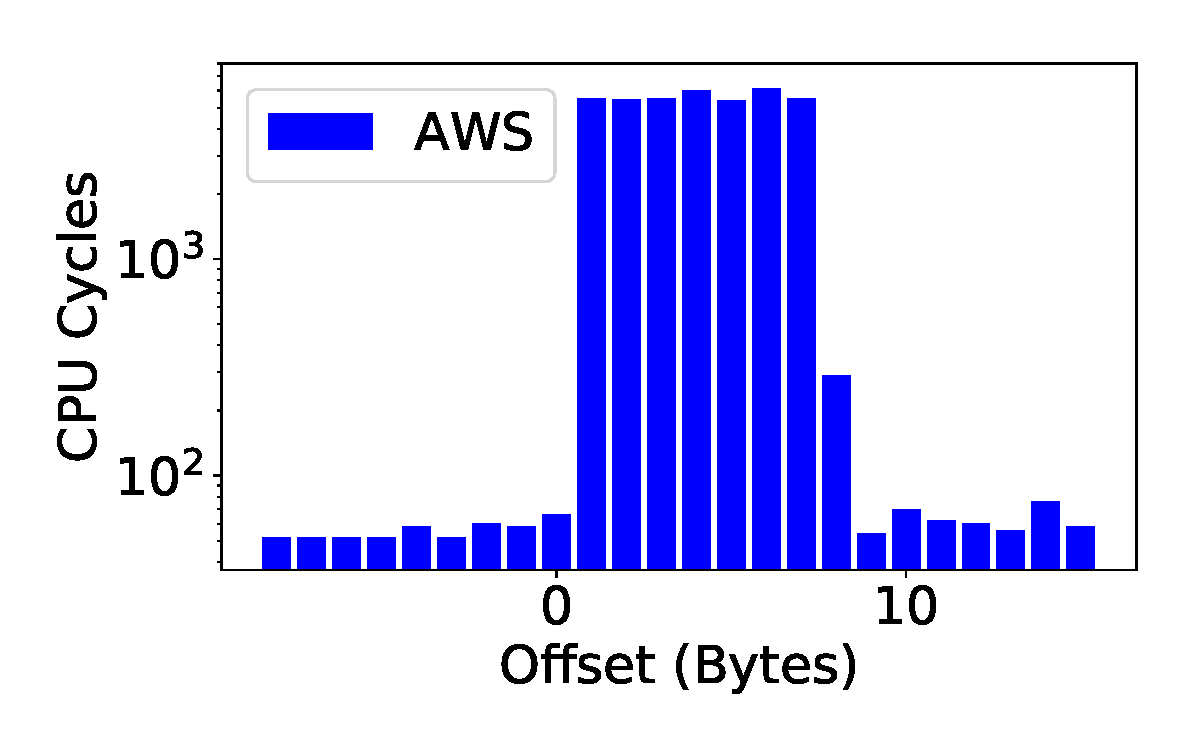
\includegraphics[width=.99\linewidth]{fig/membus_aws.pdf}
%   \caption{1a}
%   \label{fig:sfig1}
\end{subfigure}%
\begin{subfigure}{.33\textwidth}
  \centering
  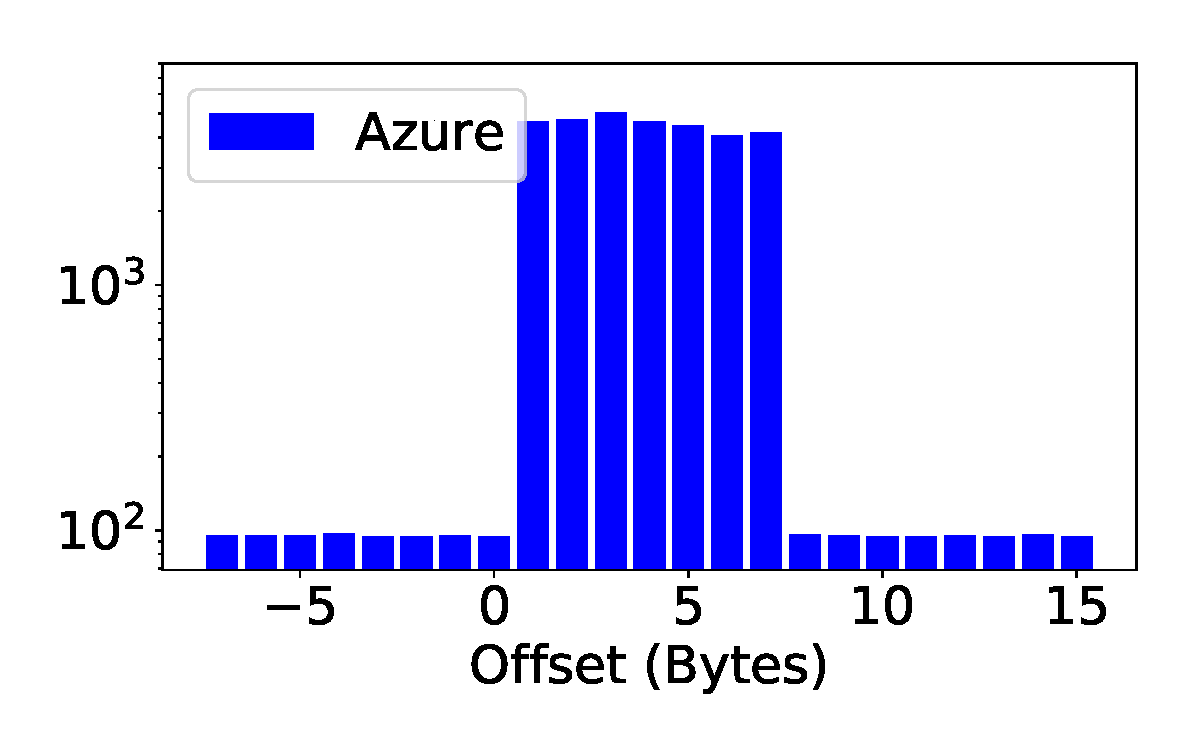
\includegraphics[width=.99\linewidth]{fig/membus_azure.pdf}
%   \caption{1b}
%   \label{fig:sfig2}
\end{subfigure}
\begin{subfigure}{.33\textwidth}
  \centering
  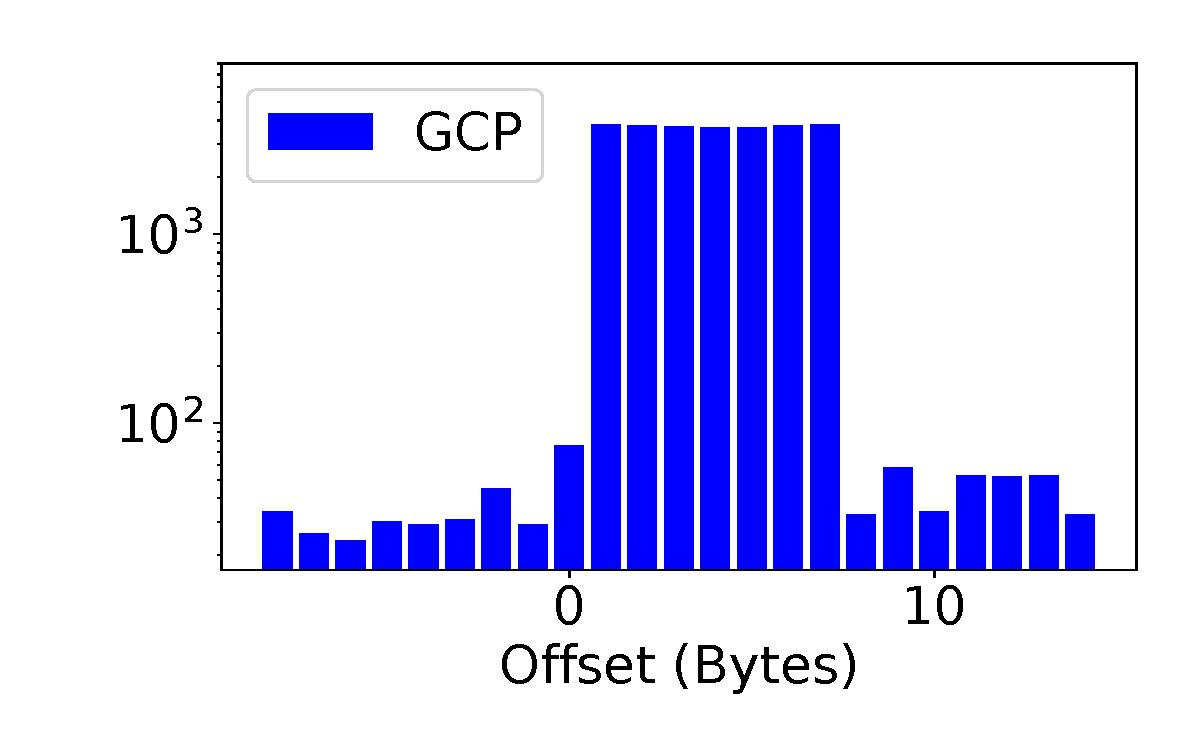
\includegraphics[width=.99\linewidth]{fig/membus_gcp.pdf}
%   \caption{1b}
%   \label{fig:sfig2}
\end{subfigure}
\caption{From left to right, the plots show the latencies of atomic 
      memory operations performed on an 8B memory region as we slide it 
      from one cache line across the boundary into another, on AWS, GCP and 
      Azure clouds respectively. \todo{Get plot for GCP}. The latencies 
      are orders of magnitude higher when the 8B region falls across the 
      two cache lines (offsets 0-7B) demonstrating the presence of 
      the memory bus covert channel on all these clouds. \label{fig:membus_clouds}}
\label{fig:fig}
\end{figure*}

% reliable - do we want to say something about this?
\amirian{make sure that all these terms are defined ahead of time: co-location,
co-operative, co-residence, serverless, lambdas}

Our goal is to determine a co-operative co-residence detection mechanism for
serverless functions. In other words, given a series of spawned lambdas in a
given region on a cloud service, how can we determine the lambdas that are
co-located on the same machines?  In this section, we discuss the details of
such a mechanism, previous solutions to this problem, and the unique challenges
we faced with lambda co-residence.

Given a set of cloud instances (VMs, Containers, Functions, etc) deployed
to a public cloud, a co-residence detection mechanism would identify, for each 
pair of instances in the set, whether the pair was running on the same physical 
server at some point. Paraphrasing Varadarajan et al.\cite{varadarajan2015}, for 
a co-detection mechanism to be useful across a wide range of 
launch strategies, we observe that it should have the following desirable 
properties:

\begin{itemize}
    \item \textbf{Generic} The technique should be applicable across a wide
    range of server architectures and software runtimes. In practice, the
    technique would work across most third-party clouds and even among different
    platforms within a cloud.
    \item \textbf{Reliable} The technique should have a reasonable detection success
    with minimal false negatives (co-resident instances not detected) and even 
    less false positives (non co-resident instances categorized as co-resident).
    \item \textbf{Scalable} A launch strategy may require hundreds or even thousands 
    of instances to be deployed, and must be fast and scalable such that the 
    technique will take less time to detect all co-resided pairs at a reasonable cost.
\end{itemize}

Given these properties, we decide to investigate harware-based covert channels.
Hardware-based covert-channels are more difficult to remove and obfuscate than
software-based covert channels, and are also more ubiquitous, given that
hardware is more homogenous in nature than software. 
% generic

\subsubsection{RNG Hardware}
\amirian{This feels a bit awkward. We might want to move this to discussion}
We first examined covert channels based on Random Number Generator (RNG)
hardware\cite{evtyushkinccs2016}.  Modern processors support this shared
hardware module to generate true random numbers. 
% These devices use low level noise signals such as thermal noise and other
% quantum phenomena to produce true non deterministic entropy. 
To produce true random numbers, information from this module is routed from the
host machine to the /dev/random file in the guest virtual machine for
cryptographic operations. Since the hardware is shared, if one guest consumes
these random bits within an infinite\amirian{does it need to be infinite?} loop,
another user could notice a spike in random operations, indicating contention on
the machine.
\amirian{do we have an old graph to back up this point of being too noisy? to
just drive the point home that RNG is not great for these purposes} 
However, our experiments on AWS using RNG hardware indicated that this channel
is unreliable for lambda co-detection. We hypothesize that perhaps, because
causing contention is easy, the channel gets too noisy as a result to accurately
use for our purposes.

% In order to get random bits, we used a Python module called rdrand that supports 
% both rdrand and rdseed instructions. While our initial plan was to run only rdseed 
% instructions which seemed better suited for our attacker logic, we found that 
% AWS hosts did not support rdseed. We also observed that rdseed was not supported 
% by few of the hosts on GCP. Hence, we run a unified program that uses rdseed
% when available and falls back on rdrand otherwise.\todo{I think we ended up 
% ditching the rdseed idea and stuck to just rdrand. (confirm just in case)} 

% We ran a simple experiment to determine if RNG techniques would be fruitful 
% for our goals. In the first run, we labeled lambdas as victims or attackers. 
% Victim lambdas would take their first set of measurements, sleep for five seconds, 
% and then take a second set of measurements. Attacker lambdas would sleep for the 
% first six seconds (long enough to allow victims to sample once without possible contention), 
% and then start "attacking". In the second run, we simply had victim lambdas run without 
% any attackers causing possible contention.  We show our results in figure~\todo{add the figure in}, 
% where the red dots are the victim lambdas that executed with the presence of attacker 
% lambdas, and the blue dots are victim lambdas that executed alone. There does not appear 
% to be a significant difference between executions when an attacker does and does not exist, 
% which indicates that RNG hardware might not be a salient avenue for determining 
% lambda co-location, as we are not able to differentiate when contention is happening.

\subsubsection{Memory bus channel}
We next explored (and ultimately used) the memory bus covert channel described
in section~\ref{sec:background:membus} as it exploits a fundamental hardware
vulnerability that is present across all generations of x86 hardware.
Historically, multiple public cloud services have been vulnerable to this
channel~\cite{varad191016,compstudycoresidency}, and we found that they are
still vulnerable today. \amirian{I think there should be another sentence or two
describing how we got to this figure right here. It sort of feels like we just
jump into results}.
Moreover, we were able to demonstrate this behavior through serverless function
instances, whose runtimes are mostly restricted to high-level languages that
prevent the pointer arithmetic required to perform these exotic operations.  To
demonstrate this attack, we used the unsafe environments (C++ on AWS, Unsafe Go
on GCP, Unsafe C\# On Azure) that these clouds allowed. 
Figure~\ref{fig:membus_clouds} shows that all three major cloud providers still
exhibit significant difference in latencies for the "exotic" memory locking
operations when compared to regular memory access latencies. This figure shows
the applicability of using memory bus across different kinds of cloud instances
as well.


% why previous approaches were not scalable
\subsubsection{Previous approaches using Memory bus}
Previous works that used the memory bus for co-residence detection divide the
deployed instances into attack and (co-operative) victim roles, and attempt to
co-locate the attacker instances with a victim instance. The attack roles
continually lock the memory bus (locking process) for a certain duration
(\textasciitilde 10 seconds) while the victims sample the memory for any spike
in access latencies (probing process). If all the deployed instances try the
detection i.e., locking and probing at once, (some of) the victims may see
locking effects, but there would be no way of knowing which or how many attack
roles co-resided with a particular victim and caused the locking. This provides
no information about the number of physical servers that ran these instances or
the amount of co-location. The only information we can deduce is that victims
were probably co-located with just a single attacker.

An alternative method is to try pair-wise detection where only one attack
instance locks and one victim instance probes at a time revealing co-residence
of this pair, and repeating this serially for each pair. However, this technique
is too slow and scales quadratically with the number of instances e.g., a
hundred instances take more than 10 hours assuming 10 secs for each pair.
\todo{get a cost estimate on ec2}. Varadarajan et al.\cite{varad191016} speeds
this process significantly by performing detection for mutually-exclusive
subsets in parallel, allowing for false-positives and later eliminating the
false-positives sequentially.\amirian{might want to elaborate on this; on its
own may be a bit confusing} This would still only scale linearly in the best
case \todo{(or not even that?)}, which is still expensive - with a thousand
instances, for example, the whole detection process takes well over 2 hours to
finish, which is infeasible for lambdas that are, by nature, ephemeral. Thus,
one challenge in this work is creating a faster neighbor detection algorithm.

% how do we scale it - challenges.
\subsubsection{The Path to Scalability}

One method to quicken the co-location process is by cutting down on the time it
takes for single attack-victim pair to determine co-residence i.e., improving
upon probing time and accuracy of the victim. However, this only affects total
time by a constant factor. To improve scalability, we need to be able to run
detection for two\amirian{why two?} attack-victim pairs in parallel without
sacrificing the certainty when they are run serially. For example, when both
pairs see co-residence, we must be certain that each victim experienced
co-residence because of its own attacker pair, which is not possible if
co-residence is ascertained based a simple yes/no signal from the attack
instance. 

The memory bus convert channel was used to exchange more complex
information like keys in previous work\cite{wuusenix2012}, and at first sight,
can be used to exchange information such as IDs between the co-resided instances
to solve our problem.  However, the original work assumes that there is only one
sender and one receiver who know exactly how and when to communicate. As we will
see in the next section, this model is not sustainable when there exist many
parties that have no knowledge of each other but try to communicate on the same
channel.

To solve some of the challenges mentioned previously, we propose a protocol in
which we use the memory busy covert channel to exchange IDs between instances,
and the co-resided instances reliably exchange their IDs with each other to
discover their neighbors. \amirian{this sentence is a bit confusing}The protocol
takes time on the order of number of instances involved, which is limited by the
maximum number of co-located instances on a single server (tens) - something
that is orders of magnitude less than total number of instances deployed to the
cloud (hundreds to thousands).  This lets us scale our co-residence detection
significantly to run in \amirian{seconds? minutes?}.

% ofcourse, this only works if all the instances are in our control 
% so we limit our focus to cooperative co-residence detection - where do 
% we add this?

\section{Neighbor Discovery Protocol}
\label{sec:technique}
 
As noted earlier, co-residence detection scales well when co-residing 
instances on each server communicate among themselves and discover each other. 
Assuming that the instances 
have unique IDs, this requires the co-resided instances to exchange these (integer) IDs with each other using the memory bus channel as a transmission medium. In this section, we present a communication protocol that the co-resided instances can use to achieve this in a fast and reliable way. We first discuss the challenges we faced in making the 
channel reliable before diving into the protocol itself.

\begin{algorithm}[!t]
\caption{Writing 1-bit from the sender}
\label{alg:sender}
\begin{algorithmic}
\STATE $now \leftarrow  time.now()$
\STATE $end \leftarrow now + sampling\_duration$
\STATE $address \leftarrow cache\_line\_boundary-2$
\WHILE{$now < end$}
    \STATE $\_\_ATOMIC\_FETCH\_ADD(address)$
    \STATE $now \leftarrow  time.now()$
\ENDWHILE
\end{algorithmic}
\end{algorithm}

\subsection{Reliable Transmission}
Consider the simple scenario where there is one sender and one receiver 
instance on a machine, and the sender has a set of bits that it needs to communicate 
with the receiver on the memory bus covert channel. On the sender side, to send 
a 1-bit the sender causes contention on the memory bus by locking it using
the special memory locking operations as discussed in section \ref{sec:background:membus} 
(pseudo-code of the sender is shown in Algorithm \ref{alg:sender}).
\todo{what is the subject here? rewrite with subject at front} Reading the bit on a 
receiver would then require sampling the memory bus for contention, 
inferring a 1-bit when the contention is observed or a 0-bit otherwise.

\subsubsection{Sensing contention} 
There are two ways in which the receivers could detect memory bus contention. 
When the memory bus is locked, any non-cached memory 
accesses will queue and therefore see higher latencies. The receiver can 
then continually make un-cached memory accesses (referred to 
as \textit{memory probing} receiver in literature\cite{varadarajan2015}) and 
observe spike in their latencies to detect contention.
The receiver could also use the same memory locking 
operations as the sender (referred to as \textit{memory locking} receiver) to 
probe the memory bus. 
Since only one processor core can lock the memory bus at a given time, any other 
concurrent locking operation will see higher latency. 

Previous studies\cite{wuusenix2012,varadarajan2015} have established that both 
memory probing and locking receivers experience significant latency overhead when compared 
to their baselines during memory bus contention, making both of them desirable 
contenders for sensing the channel on the receiver side. We examine which of the two 
would be more fruitful for our experiments. Memory probing involves regular (un-cached) 
memory accesses, which is universal, unlike the locking operations which are rarely used, 
if at all, by standard applications. This makes memory probing the only viable option 
for non-cooperative co-residence detection, where 
victims are not under attacker's control and cannot be assumed to perform locking 
operations. Furthermore, memory probing can be done on multiple receivers 
constantly without affecting each other (due to the high memory bandwidth), which prevents 
noise in measurements. This is an important attribute, as memory locking receivers 
must contend with this noise. However, bypassing multi-levels of caches in today's servers 
to perform memory accesses with reliable consistency is a challenging task 
\todo{cite some papers}. Even with a reliable cache-bypassing technique, the 
variety of cache architectures and sizes that we encounter on different clouds 
would make tuning the technique to suit these architectures an arduous task while 
reducing the applicability of our overall co-residence detection mechanism. 
Thus, we decide to use the memory locking receiver.


\begin{algorithm}[!t]
\caption{Reading a bit in the receiver}
\label{alg:receiver}
\begin{algorithmic}[1]
\STATE $now \leftarrow  time.now()$
\STATE $end \leftarrow now + sampling\_duration$
\STATE $sampling\_rate \leftarrow num\_samples / sampling\_duration$
\STATE $address \leftarrow cache\_line\_boundary-2$
\STATE $samples \leftarrow \{\} $
\WHILE{$now < end$}
    \STATE $before \leftarrow RDTSC()$
    \STATE $\_\_ATOMIC\_FETCH\_ADD(address)$
    \STATE $after \leftarrow RDTSC()$
    \STATE $samples \leftarrow samples \cup \{(after-before)\}$
    \STATE \textbf{wait until} $NEXT\_POISSON(sampling\_rate)$
    \STATE $now \leftarrow  time.now()$
\ENDWHILE
\STATE $ks\_val \leftarrow KOLMOGOROV\_SMIRINOV(samples, baseline)$
\STATE \textbf{return} $ks\_val < ksvalue\_threshold$
\end{algorithmic}
\end{algorithm}


\subsubsection{Sampling frequency}
Ideally, a memory locking receiver would perform locking operations in a loop and 
look for a dip in the moving average of the number of operations to determine
contention in real-time. Note that, in this case, there is 
essentially no difference between the sender and receiver (i.e., both continually issue
locking operations) except that receiver is taking measurements. This is adequate when 
there is a single sender and receiver~\cite{varadarajan2015},
but when there are multiple receivers, the mere act of sensing the channel by one 
receiver causes contention and other receivers cannot differentiate between a silent (0-bit) 
and a locking (1-bit) sender. To avoid this, we space the sampling of memory bus such that 
no two receivers would sample the bus  at the same time, with high probability. 
We achieve this by using large intervals between successive samples and a poisson-sampling 
to prevent time-locking of receivers. We determined that a millisecond poisson gap between 
samples is reasonable to minimize noise due to collisions in receiver sampling~\ref{fig:membus_clouds}, 
assuming ten co-resided receivers and sampling takes a few microseconds each time.

\subsubsection{Sampling duration}
\label{sec:method:samplingdur}
A receiver can confirm contention with high confidence with only a few samples, assuming 
that the sender is actively causing contention on the memory bus
and the receiver is constantly sampling the memory bus throughout the sampling duration. 
However, in practice, the time-sharing of processors produces difficulties. 
The sender is not continually causing contention, and neither is the receiver sensing it, 
as they are context-switched by the scheduler to run other processes. 
Assuming that the sender and receiver are running on different 
cores, the amount of time they are actively communicating depends on 
the proportion of time they are allocated on each core and how they are 
scheduled. 

To illustrate such behavior, we run a sender-receiver pair using 
the Lambdas\cite{awslambda} of various sizes on AWS,
and compare the distribution of latencies seen by the receiver during the 
contention in each case. Figure \ref{fig:context_switching} shows that the much smaller 
128 MB lambdas (which probably share a CPU core with others and gets constantly context-switched) 
show less active communication than the bigger 3 GB lambdas (which may run on dedicated cores). 
This means that smaller instances that tend to share
processor cores with a lot of other instances may need to pause for more time
and collect more samples to make up for lost communication due to scheduling.
% Since the typical scheduling quantum is on the order of milliseconds, they 
% will need at least a second?


\begin{figure}[!t]
  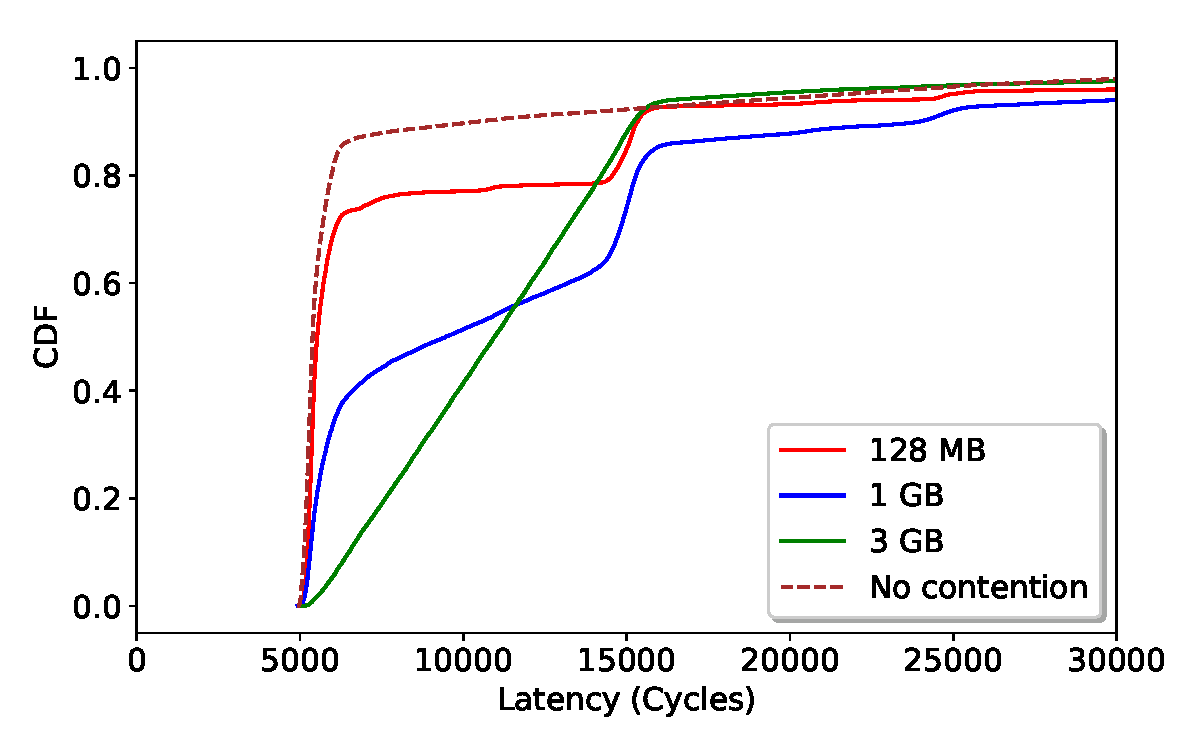
\includegraphics[width=.99\linewidth]{fig/lambda_sched_effect.pdf}
  \caption{Shows CDF of latencies observed by 128 MB, 1 GB and 3 GB Lambdas during 
  contention. The 128 MB lambda pair sees less contention due to more context switching, 
  whereas the 1 GB and 3 GB lambdas see progressively more contention compared to baseline 
  which we attribute to their relative stability on the underlying physical cores. 
\label{fig:context_switching}}
\end{figure}

\subsubsection{Overcoming noise} 
\label{sec:method:noise}
Along with context switching and sensing noise, there are other imperfections 
in measurement apparatus that cause (minor) noise. For example, we use difference
in RDTSC timer readings before and after the locking operation to measure its 
latency in cycles. If the receiver process gets context-switched in 
between the timer readings 
(e.g., at line 8 in Algorithm \ref{alg:receiver}), the latency measured from 
their difference will be orders of magnitude higher 
as it includes waiting time of the receiver process in the scheduler queue 
- which we believe is what contributes 
to the long tail in Figure \ref{fig:context_switching}. To overcome missed 
samples and noise, we take hundreds of samples for communicating each bit 
and compare it to the baseline 
distribution of latencies sampled without contention. 
We then take a variant of two-sample Kolmogorov-Smirinov (KS) test as a measure 
to differentiate observed sample of latencies from the baseline and to establish 
contention (In our variant, we take the mean of absolute difference between the 
empirical CDFs instead of the maximum). We categorize a KS-value above certain 
threshold (KS-threshold) as a 1-bit, or a 0-bit otherwise. 

To figure out whether 
such a threshold exists and a way to find it, we deploy a large number of lambdas 
across AWS regions where some of them cause contention (aka senders) while others 
observe contention by collecting samples of latencies (aka receivers). Each of the 
samples may or may not have observed contention depending on whether the receiver 
was colocated with a sender lambda (an unknown at this point). We then calculate the 
KS-value for each sample against the baseline
and plot a CDF of these values for lambdas of different sizes in Figure \ref{fig:ks_values}.
Ideally, we expect a bi-modal distribution (stepped CDF) with the lower and upper peaks 
corresponding to samples that have not and have seen contention respectively, and a big 
gap between the two (long step). Fortunately, we do see that at higher lambda sizes 
(which lets us pick a clear threshold) but is not the case with smaller lambdas where 
scheduling instability causes lossy communication, as discussed in \ref{sec:method:samplingdur}.
This also reflects in the reliability of our technique across various lambda sizes, as 
we will show in our evaluation. Based on the plot, we picked KS-threshold at 3.0 which 
seems to be constant across AWS regions, suggesting that this is a platform constant.

We present pseudo-code of a receiver in 
Algorithm \ref{alg:receiver} that includes all the 
considerations we discussed so far.

\subsubsection{Clock synchronization} 
Since communicating each bit of information takes time (i.e., receiver sampling 
duration), we need a way to synchronize sender and receiver at the start of 
each bit. In traditional analog channels, this is achieved either using a 
separate clock signal or a self-clocking signal encoding. For example, 
\cite{whispers} uses differential Manchester encoding for clock synchronization 
for the memory bus covert channel.
But self-clocking encodings  become much trickier (\ques{why?}) when there are 
multiple senders and receivers. In this work, we use the system clock in the instances 
for synchronizing communication. We make the insight that all the instances involved 
in the communication would be running on the same physical server and 
so they share the server's clock. 
The system clock on AWS Lambdas, for example, is precise up to nanoseconds 
with a sub-microsecond drift between different lambdas running on the same server,
which is by far good enough as we only work in the millisecond regime due to 
sampling noise constraints.
% this would limit application to VMs.. but containers are probably okay..


\begin{figure}[!t]
  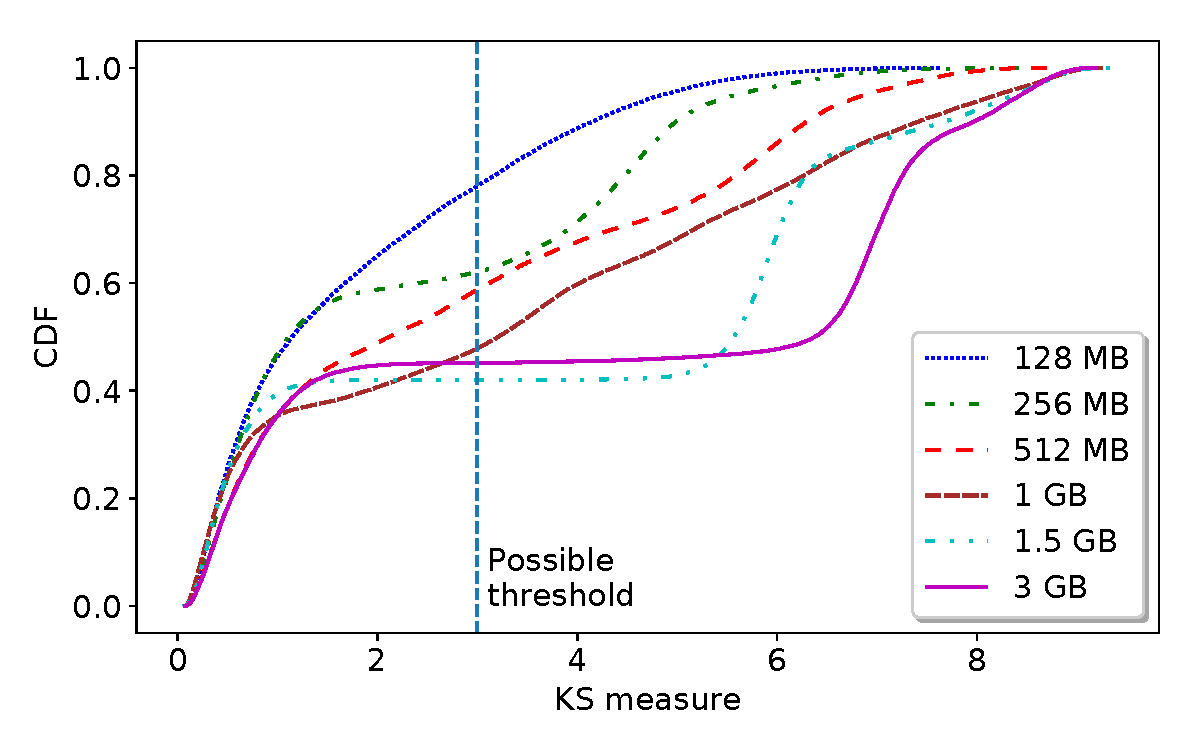
\includegraphics[width=.99\linewidth]{fig/ksvalues.pdf}
  \caption{Shows CDF of KS values observed for various lambda sizes. A bimodal distribution 
  with longer step lets us pick a KS-threshold that enables our technique to differentiate 
  between 0-bit and 1-bit with high confidence. 
\label{fig:ks_values}}
\end{figure}

\subsection{Protocol}
\label{sec:protocol}
After the previous section, what we have is a communication channel with 
synchronized time slots (called \textit{bit-slots}) where in each slot, an 
instance can reliably send (broadcast) or receive (listen) a bit by causing 
or sensing for contention respectively. Given that there are multiple instances that 
may want to 
broadcast information on the channel, we need a figure out who goes first, or 
there will be collisions. Traditional channels like Ethernet or Wireless 
detect collisions and employ random back-off to avoid them. This will be challenging 
to implement in our case for two reasons: First, our instances do not have the 
capability of sensing the channel while sending a bit, which 
is required for detecting collisions - they can either cause contention or sense 
it at a time, but not both. Note that senders do experience a push back 
(i.e., higher latency for locking operations) where there are other senders that 
are simultaneously causing contention. However, reliably judging this push back 
requires each sender to have a baseline of latencies collected when there are 
no collisions, making it a chicken-and-egg problem for avoiding collisions. 
Second, even if we use random back-offs with acknowledgement based techniques, it 
adds a lot of overhead before any meaningful communication happens - which is 
only made worse as the number of instances involved grows. Note that each bit-slot 
takes up to 1 second, so the additional overhead can be really high. \anil{get 
information theoretic bounds on the capacity of our channel?}


\begin{algorithm}[!t]
\caption{ID exchange protocol \todo{Improve pseudo-code}}
\label{alg:protcol}
\begin{algorithmic}[1]
\STATE $sync\_point \leftarrow$ {Start time for all instances}
\STATE $ID \leftarrow$ {Instance ID}
\STATE $N \leftarrow$ {Number of bits in ID}
\STATE $advertising \leftarrow TRUE$
\STATE $instances \leftarrow \{\} $
\STATE $WAIT\_TILL(sync\_point)$
\WHILE{$id\_read$}
    \STATE $slots \leftarrow 0$
    \STATE $id\_read \leftarrow 0$
    \STATE $participating \leftarrow advertising$
    \WHILE{$slots < N$}
        \STATE $bit \leftarrow$ {$slots^{th}$ most significant bit of ID}
        \IF{$participating$ \textbf{and} $bit$}
            \STATE $WRITE\_BIT()$               (Alg. \ref{alg:sender})
            \STATE $bit\_read \leftarrow 1$
        \ELSE
            \STATE $bit\_read \leftarrow READ\_BIT()$       (Alg. \ref{alg:receiver})
            \IF{$bit\_read$}
                \STATE $participating \leftarrow FALSE$
            \ENDIF
        \ENDIF
        \STATE $id\_read \leftarrow 2 * id\_read + bit\_read$
        \STATE $slots \leftarrow slots + 1$
    \ENDWHILE
    \IF{$id\_read = ID$}
        \STATE $advertising \leftarrow FALSE$
    \ENDIF
    \STATE $instances \leftarrow instances \cup \{id\_read\}$
\ENDWHILE
\STATE \textbf{return} $instances$
\end{algorithmic}
\end{algorithm}

For the co-residence detection though, we don't need the communication channel to 
be very general and expressive. So we make a simplifying assumption that each instance 
involved just has a unique fixed-length (say \emph{n}) bit-string corresponding 
to its ID that it needs to communicate with others, so we propose a communication 
protocol to exchange just this information while allowing for collisions. We 
divide the entire time that the protocol takes into phases, with each phase running 
for an interval of
\textit{n} bit-slots. Each phase has a set of participating instances, 
which in the first phase would be all of the co-located instances. In each bit-slot
\textit{k} of \textit{n} slots in a phase, every participating instance broadcasts 
a bit if $k^{th}$ bit of its 
bit-string (ID) is 1, otherwise it just listens for a 0 or 1. If an instance senses a 1 
while listening, it stops participating, and just listens for the rest of the 
phase. The result is, only the instances with highest ID among the initial 
set of participating lambdas wins out and keeps participating till the end, 
effectively advertising its ID to the rest. The advertised instance then stops 
participating in the later phases, allowing the next highest instance to advertise its 
ID, and so on. Since the IDs are unique, there will always be one instance that 
wins (and drops out) in every phase, and the protocol ends after \textit{x} phases 
(where \textit{x} is number of co-located instances) when there is no participating 
instances and everyone hears nothing for \textit{n} consecutive bit-slots. A 
pseudo-code of the protocol is provided in Algorithm \ref{alg:protcol}. Note that 
the protocol itself is channel-agnostic and can be extended for other (future) covert 
channels with similar channel properties.

% Figure moved here for formatting
\begin{figure}[!t]
  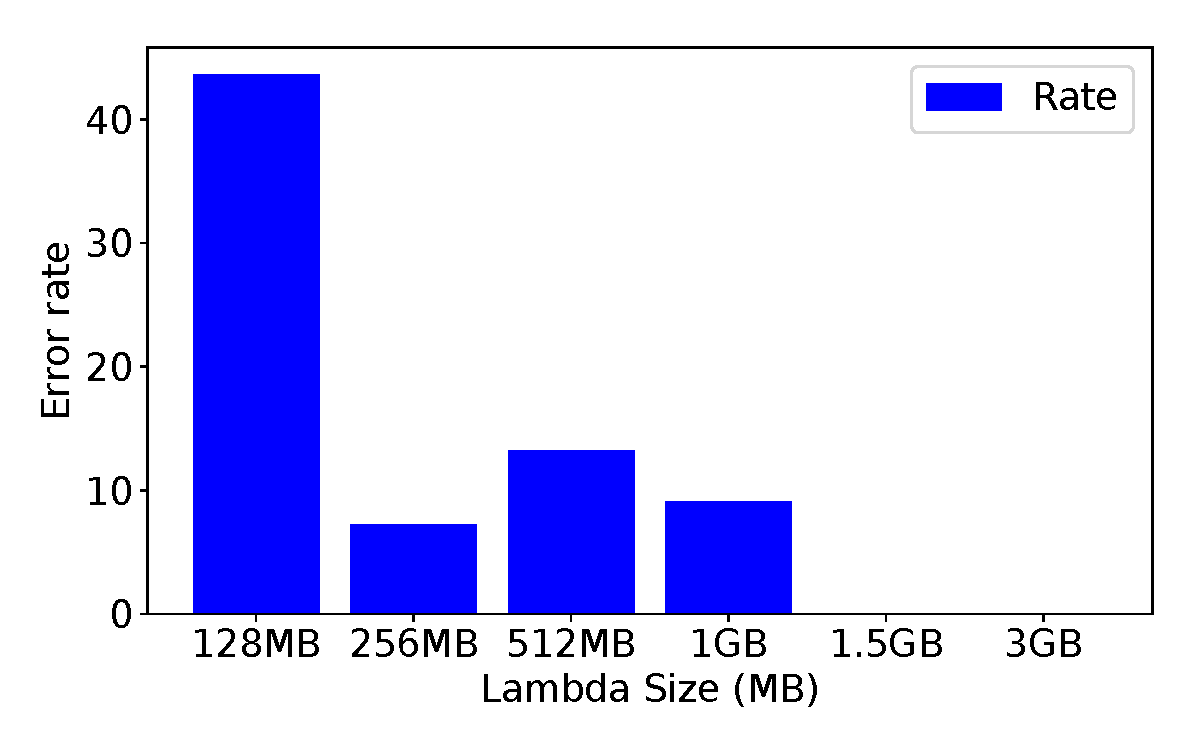
\includegraphics[width=.99\linewidth]{fig/errorrates.pdf}
  \caption{Shows the error rate (as a fraction of 1000 lambdas deployed) for different lambda sizes in AWS Middle-East region. 
\label{fig:errorrates}}
\end{figure}

\subsubsection{Complexity}
\label{sec:protocol:complexity}
Assuming \textit{N} total deployed instances to the cloud, the bit-string would need 
$\log_2N$ bits to uniquely identify each instance. If a maximum \textit{K} of those instances 
end up on the same server, the protocol runs for \textit{K} phases of $\log_2N$ bit-slots 
each, taking $(K+1)*\log_2N$ bit-slots for the whole thing. For example, assuming 10,000 deployed lambdas and a maximum of 10 co-located instances on each server, the entire  
co-residence detection takes around 4 minutes with 1-second bit-slots. 
In fact, it is not necessary to run the protocol for all \textit{K} phases. After the 
first round, all the co-located instances would know one of their neighbors. Since IDs are
globally unique, the instances can exchange it offline (through network) and figure out 
rest of their neighbors. This removes the dependency on number of co-located instances 
(\textit{K}) and brings down the complexity to $O(\log_2N)$, finishing the entire protocol 
within a minute for the earlier example!


% \subsubsection{Limitations}
% challenge with same core scheduling. - write a list of drawbacks?
% this could be overcome by getting 
% redundant info and constructing 
% the graph

\section{EVALUATION}
\label{sec:eval}

\begin{figure}[!t]
  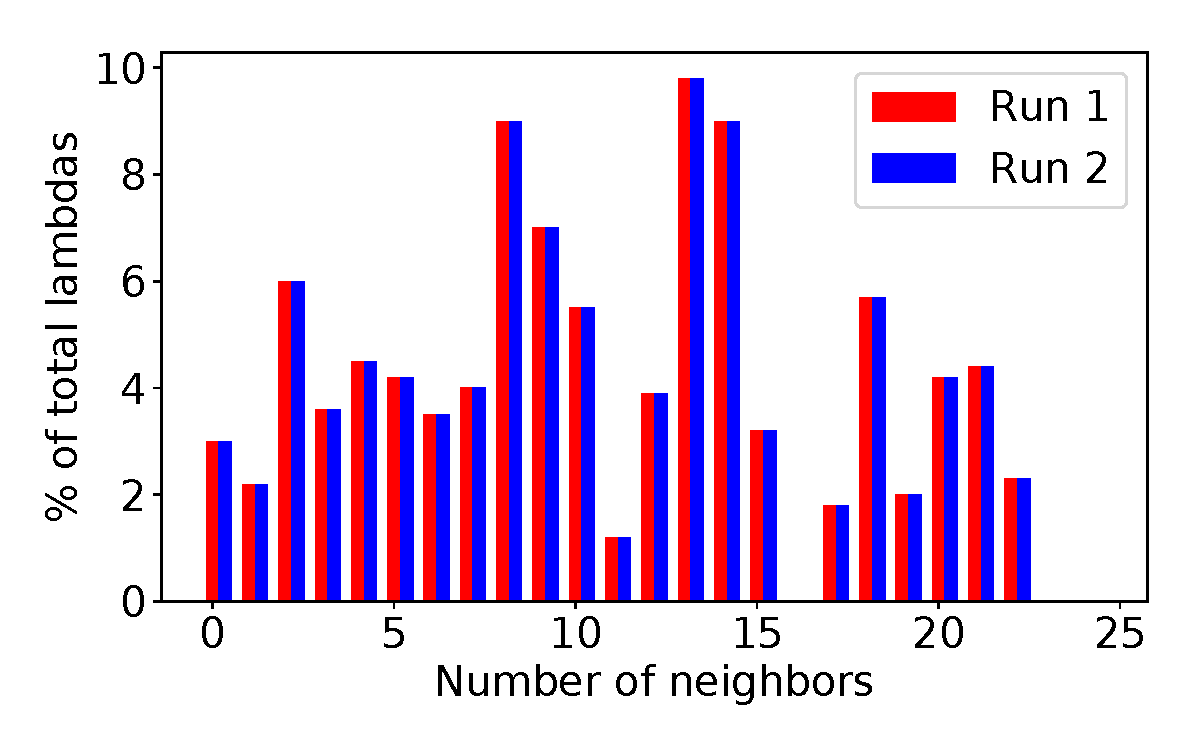
\includegraphics[width=.99\linewidth]{fig/correlation.pdf}
  \caption{Shows the fraction of lambdas by the number of neighbors they saw for two 
  independent runs that use same set of underlying AWS containers. The perfect correlation 
  shows that both runs depict the colocation status of those containers regardless of the 
  lambdas that ran on them, 
  providing an evidence for the correctness of our technique. \todo{this doesn't show perfect 
  correlation because only 99\% of lambdas warm started. Get another perfect run?}
\label{fig:correlation}}
\end{figure}

In this section, we evaluate the effectiveness of our co-residence detection 
technique with respect to the desirable properties mentioned in section \ref{sec:methodology} 
i.e., reliability and scalability. 

\subsection{Setup}
\label{subsec:expsetup}
We run all our experiments with AWS\cite{awscloud} lambdas. (We have showed that this covert 
channel exists on other clouds and so can be easily replicated with their serverless functions).
Activating the memory bus covert channel requires address manipulation using pointers and 
is not supported by most serverless platform runtimes that only allow high-level languages like Python. 
However, we were able to find at least one exception to this on all clouds: AWS allows 
C++ programs while Azure and GCP allow unsafe versions of C\# and Golang respectively.
Once deployed, each instance participates in the first phase of the protocol
as noted in section \ref{sec:protocol:complexity}, thereby learning the ID of their 
biggest neighbor. As bit-flip errors are possible, we repeat the same phase for two 
more (independent) rounds and take the majority result to record the ID seen by this instance. 
If all three rounds resulted in different IDs, we classify this instance as erroneous 
and report it in the error rate. We group all the successful instances that saw the same ID 
as neighbors. We repeat the experiments for different lambda sizes and in various cloud regions.


\subsection{Reliability}
We consider the results of the technique reliable when 1) most of the deployed instances
successfully see the same result in majority of the independent rounds (indicating 
lesser bit-flip errors) and 2) the resulting co-located groups we see match the ground truth.
For 1, we ran an experiment with 1000 AWS lambdas and compared the error rate across 
different lambda sizes (the error rate indicates the fraction of these 1000 lambdas that 
did not have a majority result). From figure \ref{fig:errorrates}, we can see that smaller 
lambdas see lot more errors. This is expected because, as discussed in section \ref{sec:method:noise}, these lambdas experience lossy communication making it harder 
for our technique to 
sense contention. The lambdas above 1.5 GB though see a 100\% success rate.   

\textbf{Correctness} Obtaining the ground truth on which instances were 
"actually" co-located is not possible, 
considering that that is the purpose of our technique. However, we found a way to 
validate our results with high confidence. AWS caches the containers used to run 
lambdas for a while (\todo{how long?}) to reuse them\cite{awscontainerreuse} for later lambdas and mitigate cold start latencies. For C++ lambdas, we found that the data structures declared in
global namespace are tied to containers (and are not cleared on each lambda invocation),
so we can use a global array to record all the 
lambdas that were ever run in a particular container. This means, for a given lambda, we can 
precisely tell all the lambdas that previously ran in the same container (aka predecessors).
Using this, we validated that identical experiments repeated within a few minutes of each 
other will use the same set of underlying containers for running the deployed lambdas.
Since the lambda co-location is essentially co-location of their containers and given that 
these containers persist across experiments (run within few minutes of each other), co-location 
results from such experiments must agree on the co-location of their underlying
containers. 




\begin{figure}[!t]
  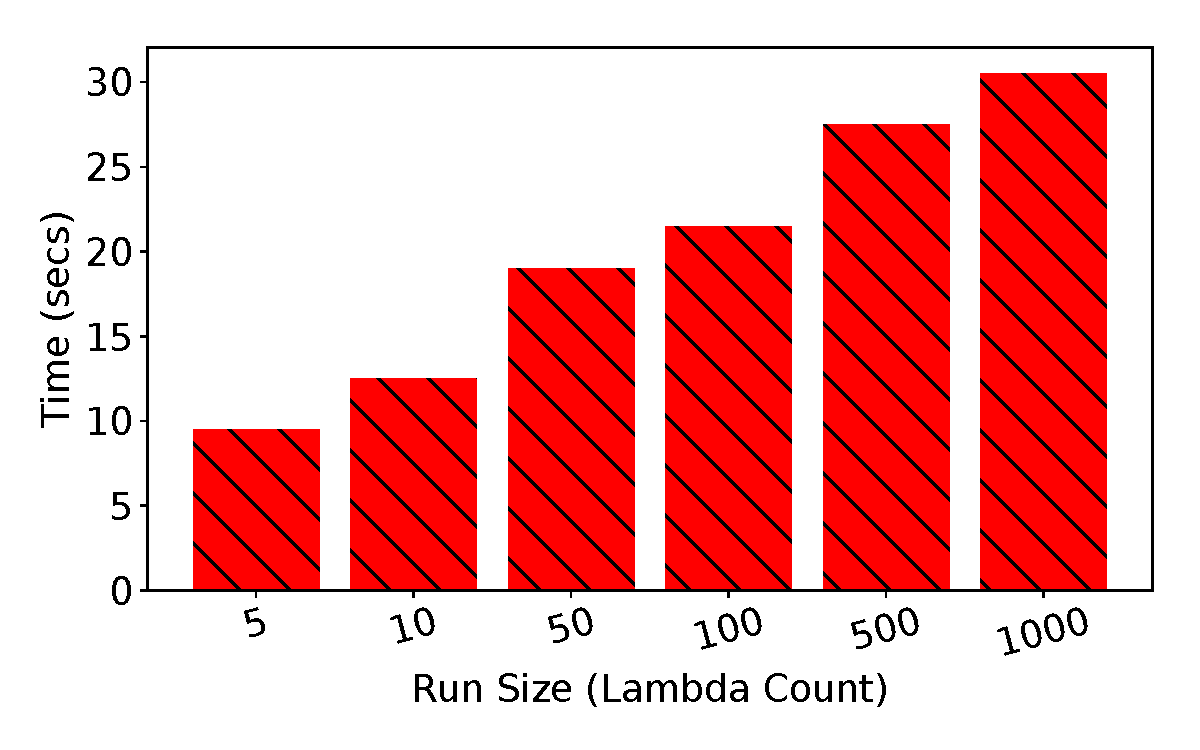
\includegraphics[width=.99\linewidth]{fig/runtimes.pdf}
  \caption{Shows the average runtime of a lambda for co-location runs of different sizes. 
  The run time increases logarithmically with the number of lambdas as it is proportional to
  the number of bits required to uniquely identify all the lambdas. \todo{Get real data.}
\label{fig:runtimes}}
\end{figure}



To demonstrate that this is the case, we run an experiment with 1000 1.5GB cold-started lambdas (ID'ed 1 to 1000) in the
one of densest AWS regions (AWS MiddleEast), which resulted in many co-located groups. 
We repeat the experiment within few seconds, making sure that all 1000 lambdas are 
warm-started this time (i.e., they use the same set of containers from the previous experiment).
For each co-located group of lambdas in the latter experiment, we checked whether their 
predecessor lambdas in the former one formed a co-located group a well. We note that while 
different lambdas used the containers across the experiments, their co-located groups 
are perfectly correlated. Figure \ref{fig:correlation} shows that both experiments saw the same 
number of groups of different sizes. This proves the correctness of our co-location results.




\subsection{Scalability}
One of the key properties of this technique is that it's really fast.
It takes only a second to communicate each binary bit of the ID, enabling 
it to scale logarithmically with the number of lambdas involved. Figure 
\ref{fig:runtimes} shows this for experiments involving different number 
of lambdas. For a run with 10000 lambdas for example, each lambda can 
find it's neighbors within a minute of its invocation, leaving ample time 
to perform other things using this information. This also means the cost 
per lambda also scales logarithmically, making it very cost-effective.



% Figures from the next section
% Moved here for formatting

\begin{figure}[!t]
  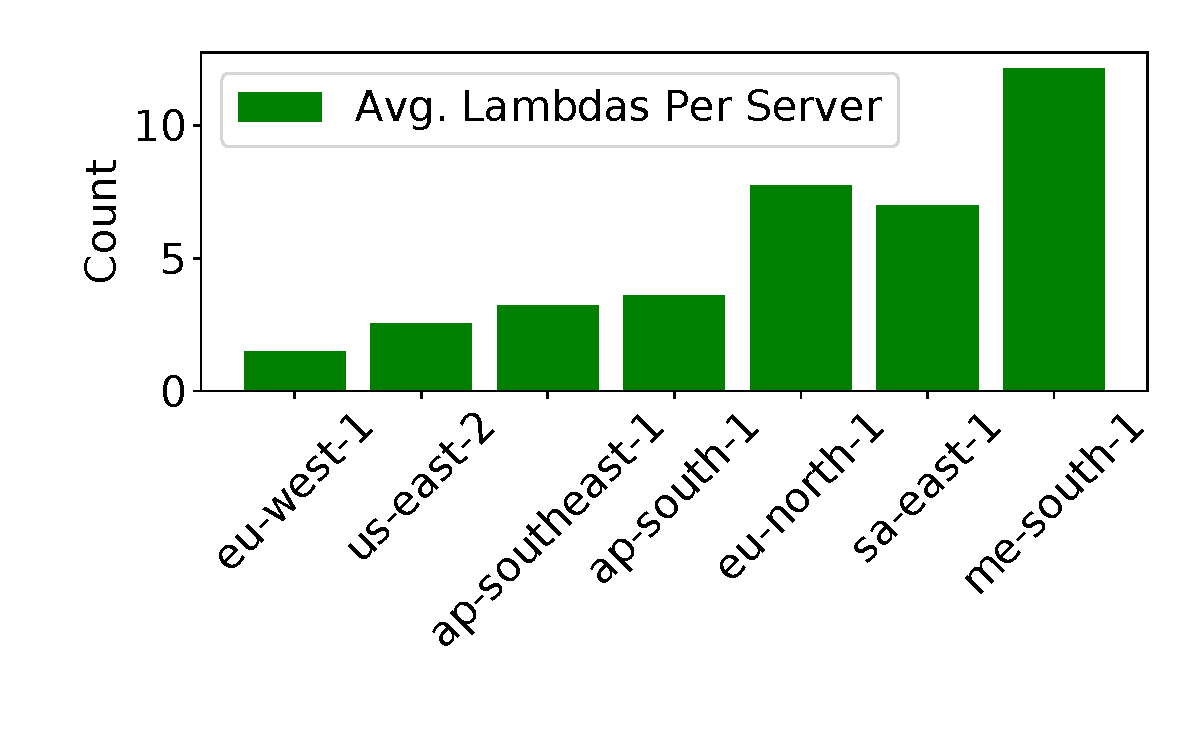
\includegraphics[width=.99\linewidth]{fig/density.pdf}
  \caption{Shows the average number of lambdas per server i.e., colocation 
  density seen in various AWS regions for a 1000-lambda run.
\label{fig:density}}
\end{figure}

\begin{figure*}[!t]
\begin{subfigure}{.33\textwidth}
  \centering
  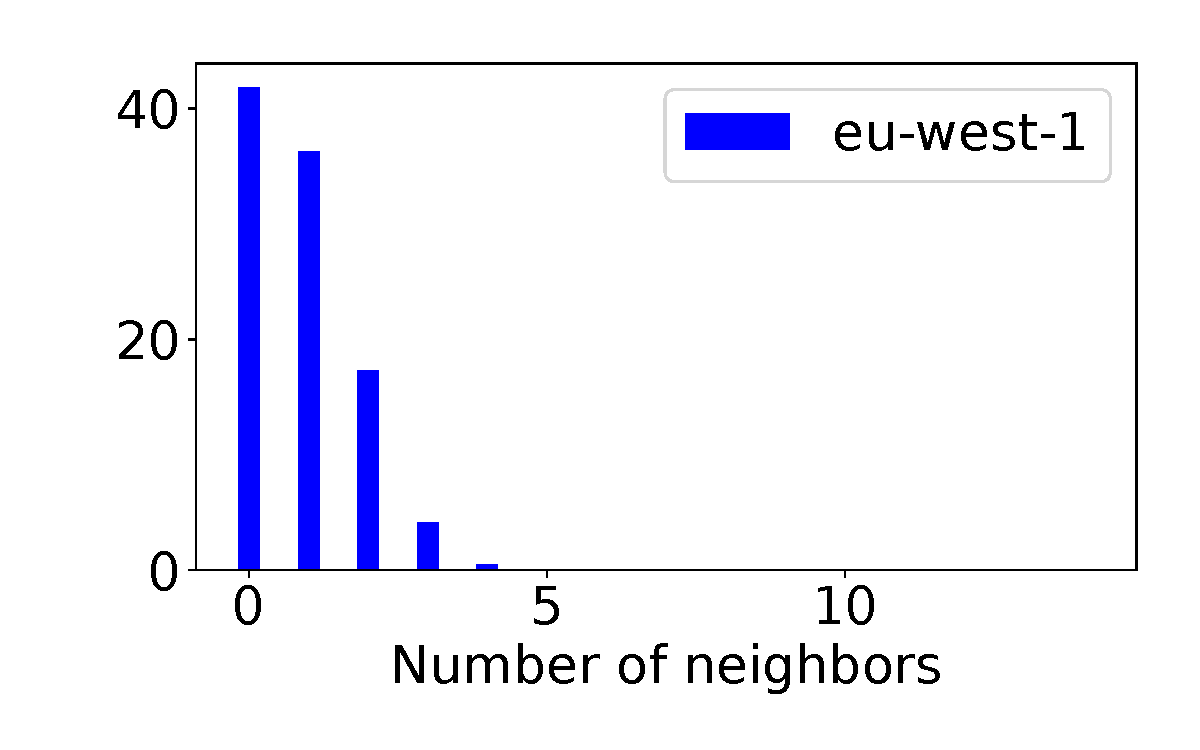
\includegraphics[width=.99\linewidth]{fig/colocation-eu-west-1.pdf}
%   \caption{1a}
%   \label{fig:sfig1}
\end{subfigure}%
\begin{subfigure}{.33\textwidth}
  \centering
  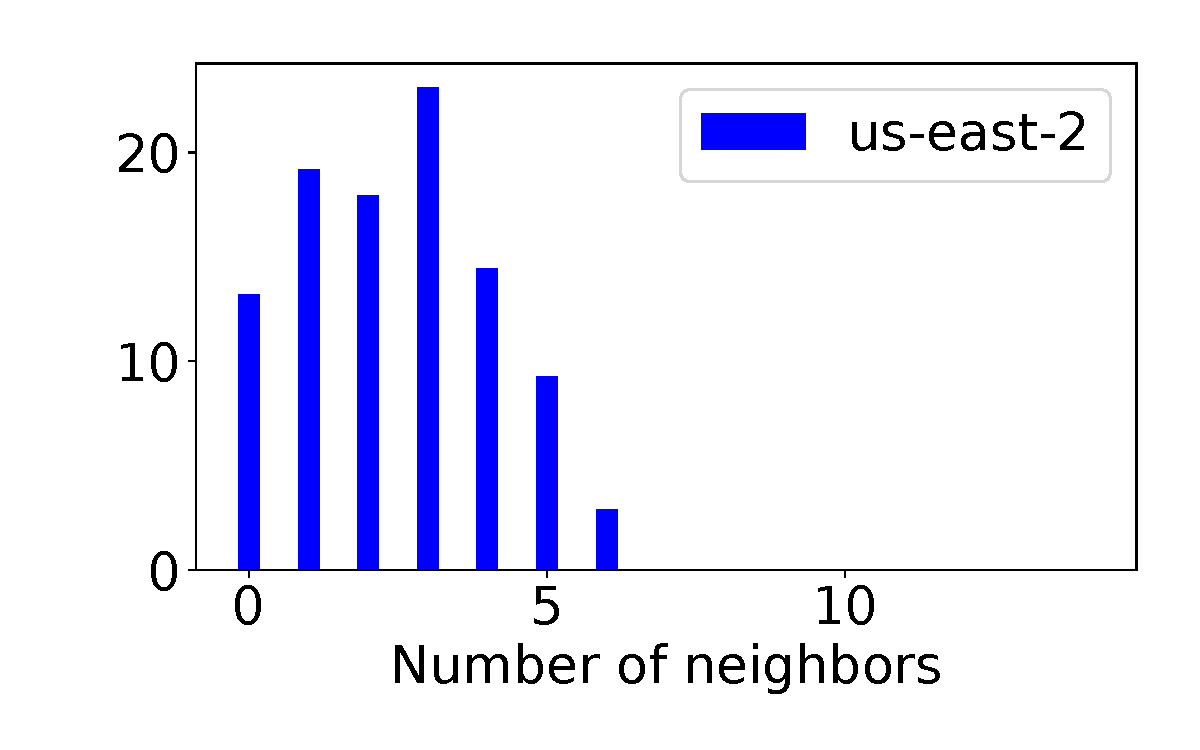
\includegraphics[width=.99\linewidth]{fig/colocation-us-east-2.pdf}
%   \caption{1b}
%   \label{fig:sfig2}
\end{subfigure}
\begin{subfigure}{.33\textwidth}
  \centering
  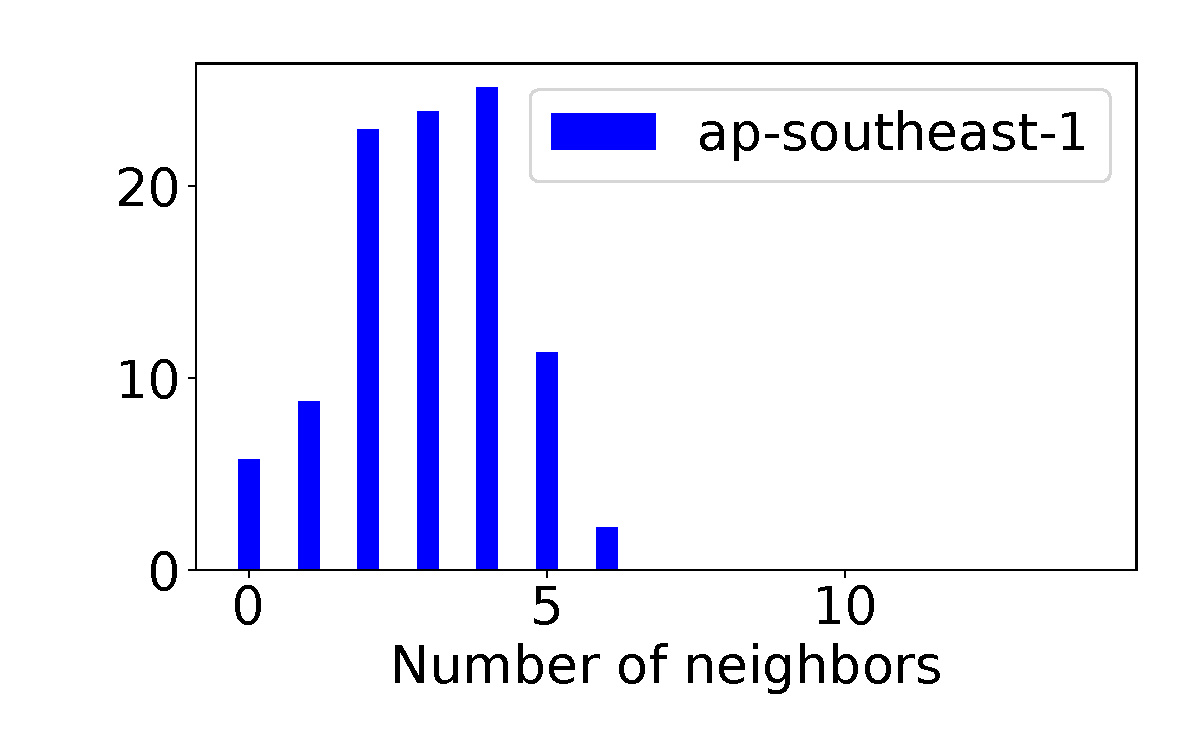
\includegraphics[width=.99\linewidth]{fig/colocation-ap-southeast-1.pdf}
%   \caption{1b}
%   \label{fig:sfig2}
\end{subfigure}

\begin{subfigure}{.33\textwidth}
  \centering
  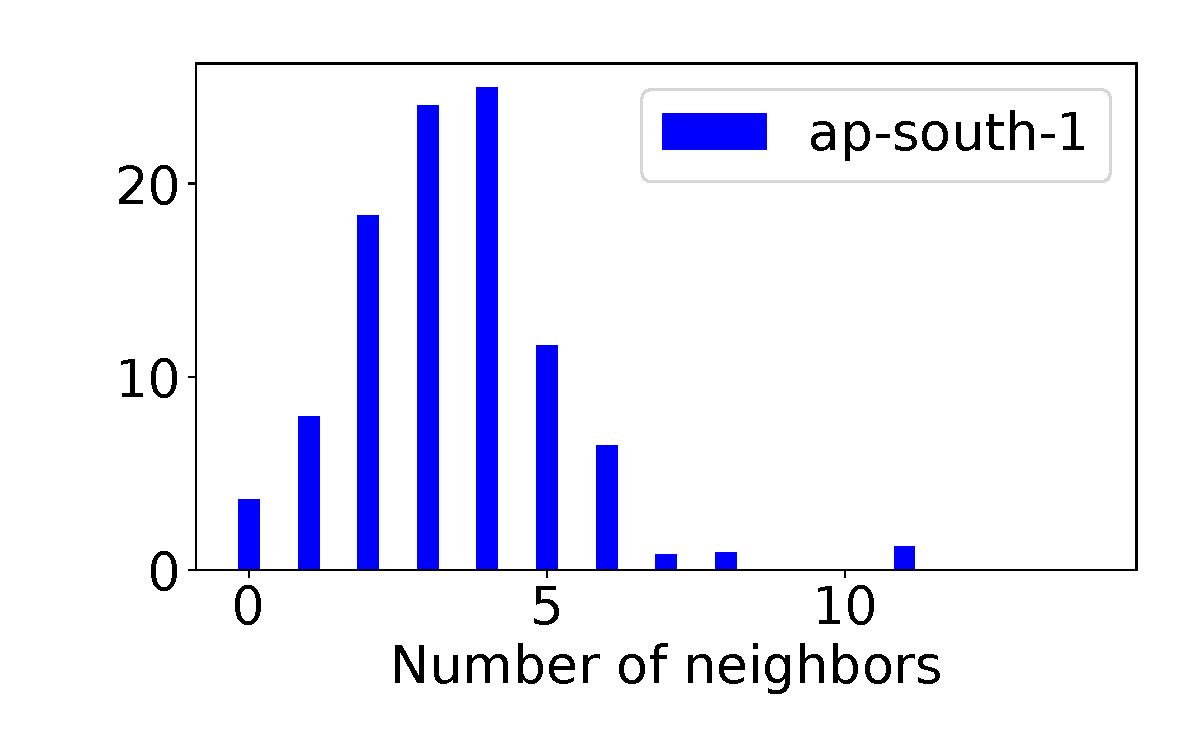
\includegraphics[width=.99\linewidth]{fig/colocation-ap-south-1.pdf}
%   \caption{1a}
%   \label{fig:sfig1}
\end{subfigure}%
\begin{subfigure}{.33\textwidth}
  \centering
  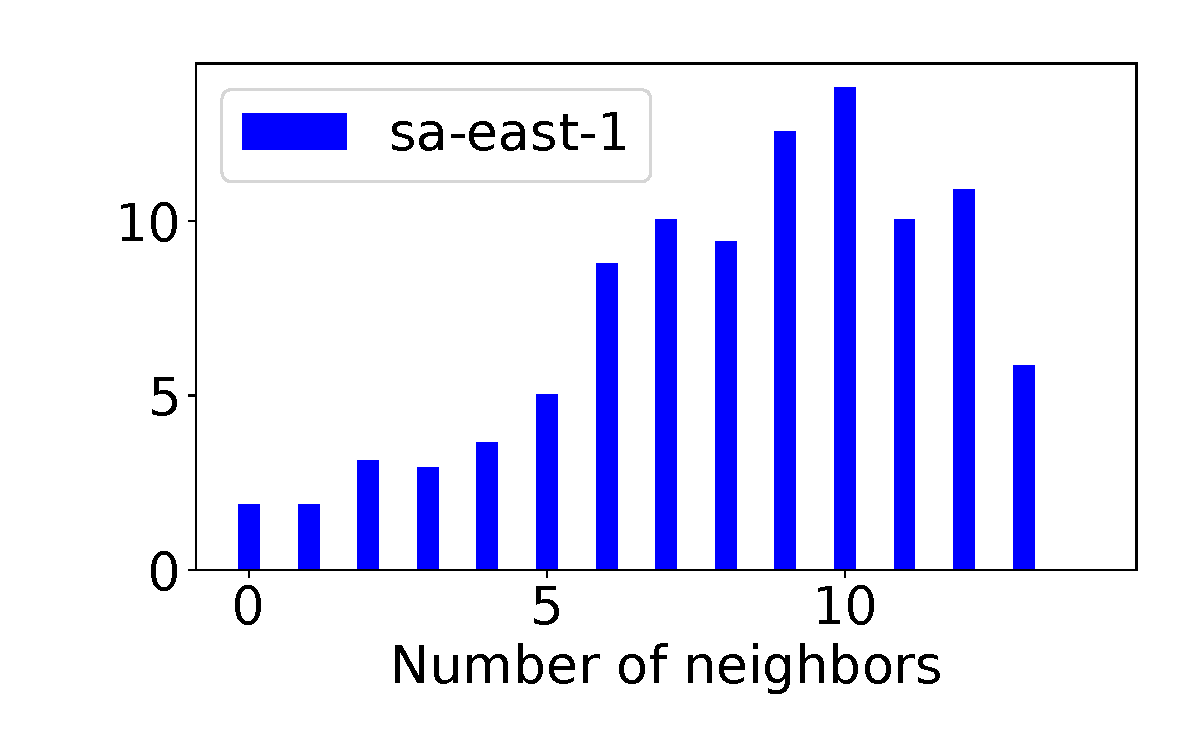
\includegraphics[width=.99\linewidth]{fig/colocation-sa-east-1.pdf}
%   \caption{1b}
%   \label{fig:sfig2}
\end{subfigure}
\begin{subfigure}{.33\textwidth}
  \centering
  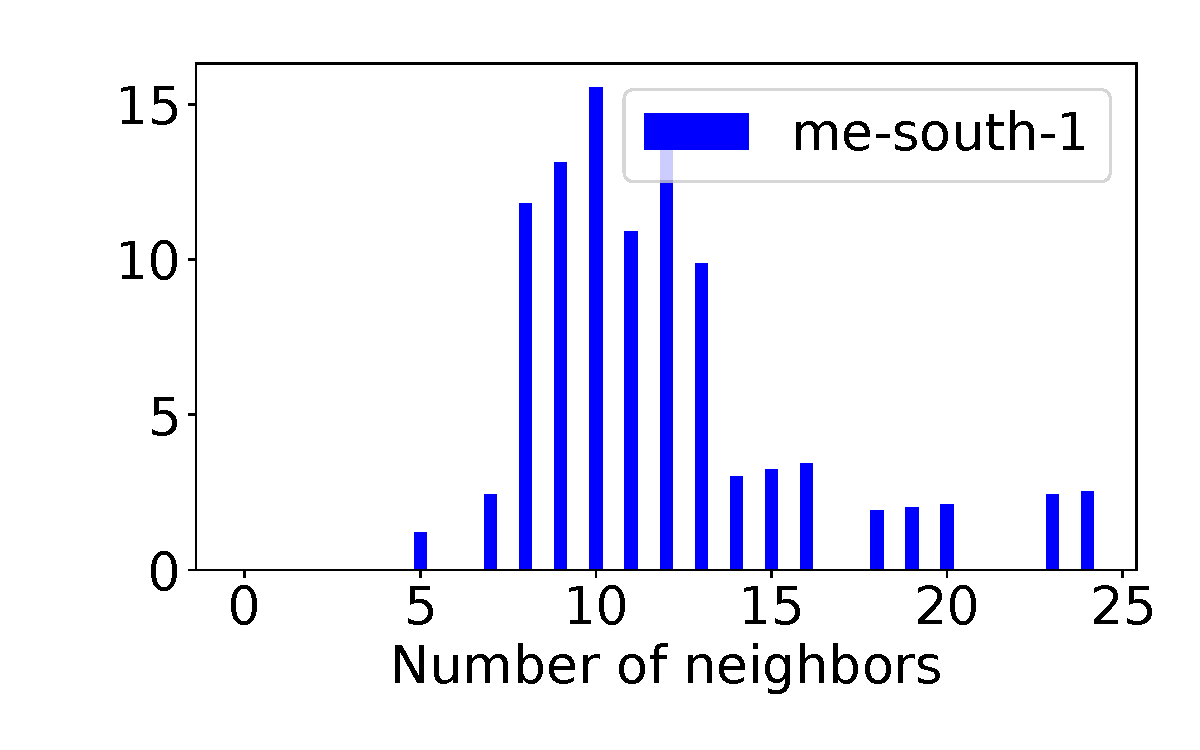
\includegraphics[width=.99\linewidth]{fig/colocation-me-south-1.pdf}
%   \caption{1b}
%   \label{fig:sfig2}
\end{subfigure}
\caption{Shows co-location results for a 1000-lambda run in different AWS regions. Each bar shows the fraction 
of those 1000 lambdas (in \%) that saw a certain number of neighbors. The total amount and density of co-location 
vary widely across regions, perhaps based on the size and lambda activity within those regions. }
\label{fig:awsregions}
\end{figure*}


%\paragraph{Generality}
%\todo{We only implemented it on AWS. This requires us to implement it on 
%Azure and GCP, and report some results. \textbf{Needs considerable effort}}

\section{Practicality of Covert Communication}
\label{sec:study}

In this section, we perform a study to demonstrate the practicality of data 
transfer using the lambda covert channels discovered with our co-residence detector.  
The amount of information that can be transferred depends on two factors: 1) the 
capacity of each channel and 2) the number of co-resident clusters of lambdas, 
or rendezvous points, that materialize during the attack.  We first produce an estimate on the
capacity of the covert channels established, and then examine the co-residence
density in various AWS regions to understand the number of rendezvous points and
factors that affect it.

\subsection{Covert Channel Capacity}


Once co-residence between any two lambas is established, the attacker can then
use the same memory bus hardware to perform covert communication. Wu et
al.~\cite{wuusenix2012}, who first introduced covert channel based on this
hardware channel, also presented an efficient and error-free communication
protocol targeting cloud-based platforms like VMs.  While such a protocol should
theoretically work for lambdas, extending it is beyond the scope of this work.
We do, however, use a much simpler (albeit more inefficient) protocol to report
a conservative estimate of the capacity of each covert channel.

Our protocol for data transfer uses the bus contention in the same way as the co-residence
detector in section \ref{sec:method:impl} to send and receive bits and perform clock
synchronization. However, now that we can use our co-residence detector to identify
lambdas on a machine and target the two that we wish to label as the sender and
receiver, we are not concerened about noise from multiple receivers, and as such
can allow the receiver to sample continuously (section \ref{sec:method:listen:freq}) 
and sample for extremely small duration (milliseconds instead of seconds). While we want the
sampling duration to be as small as possible (in order to increase the rate of
bits transferred), the chances of erasures or errors also increases as the
sender and receiver may get descheduled during this time. 

To demonstrate this, we launched hundreds of 3 GB lambdas on AWS and use our
co-residence detector to establish tens of covert channels. We then send data
over these channels at various bitrates and record the error ratio (for
byte-sized data segments). Figure~\ref{fig:channel} shows the mean error ratio
at 50\% and 95\% one-sided confidence intervals, both of which increase with the bitrate.


To correct these errors, we use Reed-Solomon coding, a block-based error correction 
code that is suitable for burst-errors caused by descheduling~\cite{wuusenix2012}. 
However, error correction comes with an overhead; With byte-sized symbols,
Reed-Solomon requires twice as many parity bytes as there are errors to correct. 
So, for each bitrate, we must compute
effective bitrate by subtracting the overhead of error correction bytes.
%required to correct its corresponding 95\% error. 
From Figure~\ref{fig:channel}, we can see that effective bitrate rises to a
maximum of over 200 bits per second (bps) (at 500 bps raw rate) before falling
again due to high error rate. We confirmed this by sending Reed-Solomon encoded
data over the covert channels at this rate and observed near-zero data
corruption. Thus, we conclude that, by a conservative estimate, we can safely
send data across each of these covert channels at a rate of ~200 bps.



\begin{figure}[!t]
  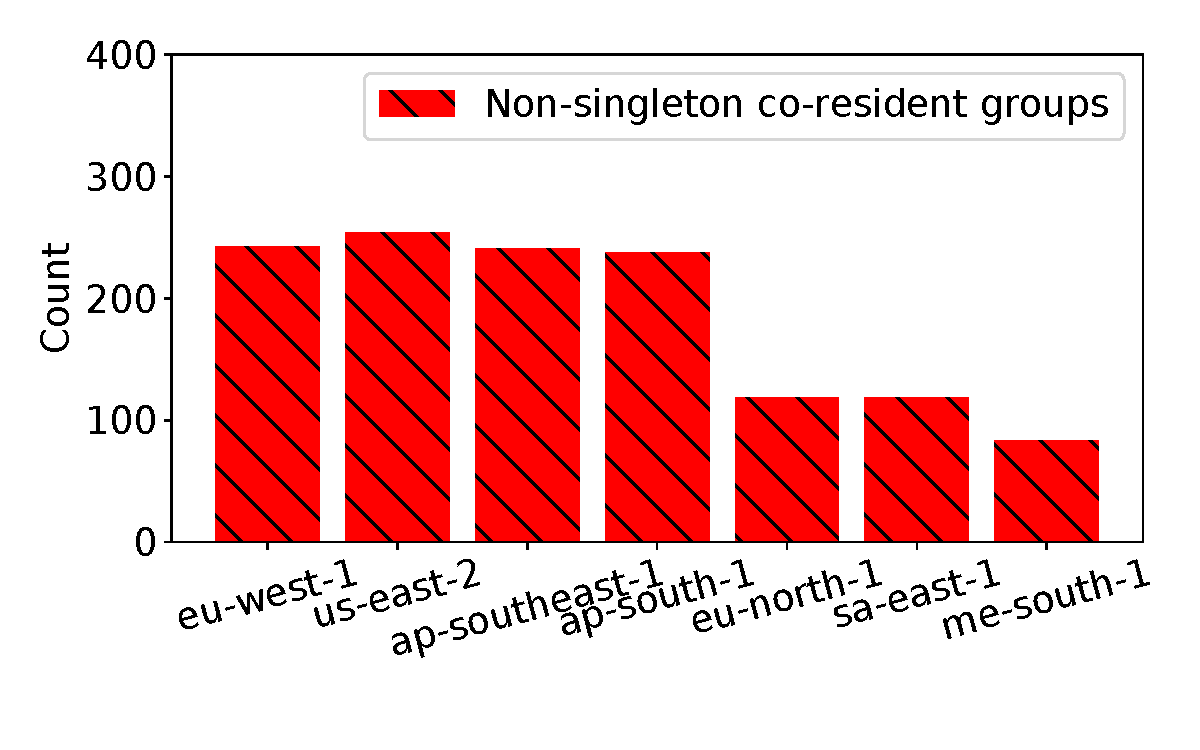
\includegraphics[width=.99\linewidth]{fig/clusters.pdf}
  \caption{This figure shows the number of co-resident groups with more than two lambdas
  seen in various AWS regions for the runs shown in Figure~\ref{fig:awsregions}. 
  Each such co-resident group can host a covert channel, indicating that a 1000 lambda 
  deployment can enable hundreds of covert channels.
\label{fig:clusters}}
\end{figure}


\subsection{Covert Channel Density}
Finally, we present measurements on covert channel density on AWS using our
co-residence detector, and discuss the factors that may affect this density.  As
we discussed in section \ref{sec:motivation}, each co-resident group of lambdas 
represent an individual server in the cloud and hence can enable an independent 
covert channel whereever the group has more than two lambdas. So we attempt to answer 
the following question: assuming that the user launches a number of
(sender and receiver) lambdas at a specific point in time, what is the expected
number of such co-resident groups (with two or more lambdas) that they might see? 
We deploy a large number of lambdas on various AWS regions and report the co-residence 
density, that is, the average number of such co-residence groups. The higher the 
co-residence density, the easier it is for the user
to ultimately establish covert channels with lambdas, and the more information
they can send. Unless specified otherwise, all the experiments discussed in this
section are performed with 1.5 GB lambdas and executed successfully with
\textbf{zero error} in co-residence detection.


\begin{figure*}[!t]
    \begin{subfigure}{.5\textwidth}
      \centering
      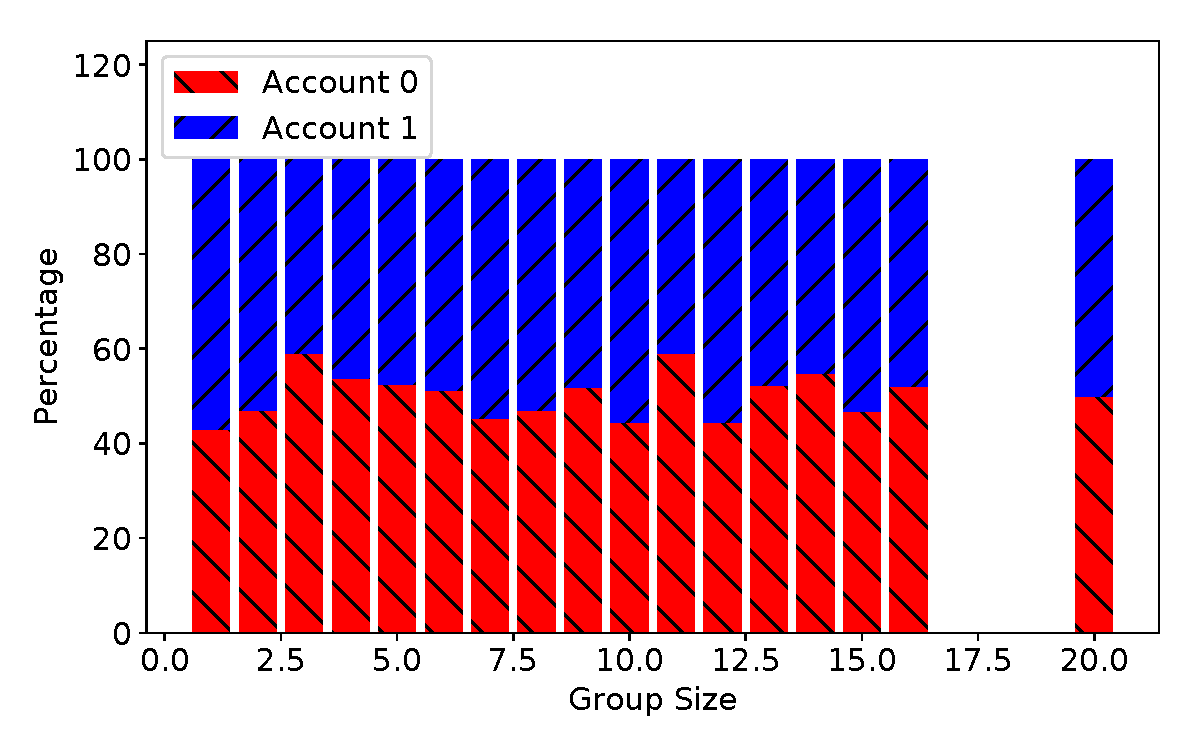
\includegraphics[width=.99\linewidth]{fig/different-accounts.pdf}
    %   \caption{1a}
    %   \label{fig:sfig1}
    \end{subfigure}%
    \begin{subfigure}{.5\textwidth}
      \centering
      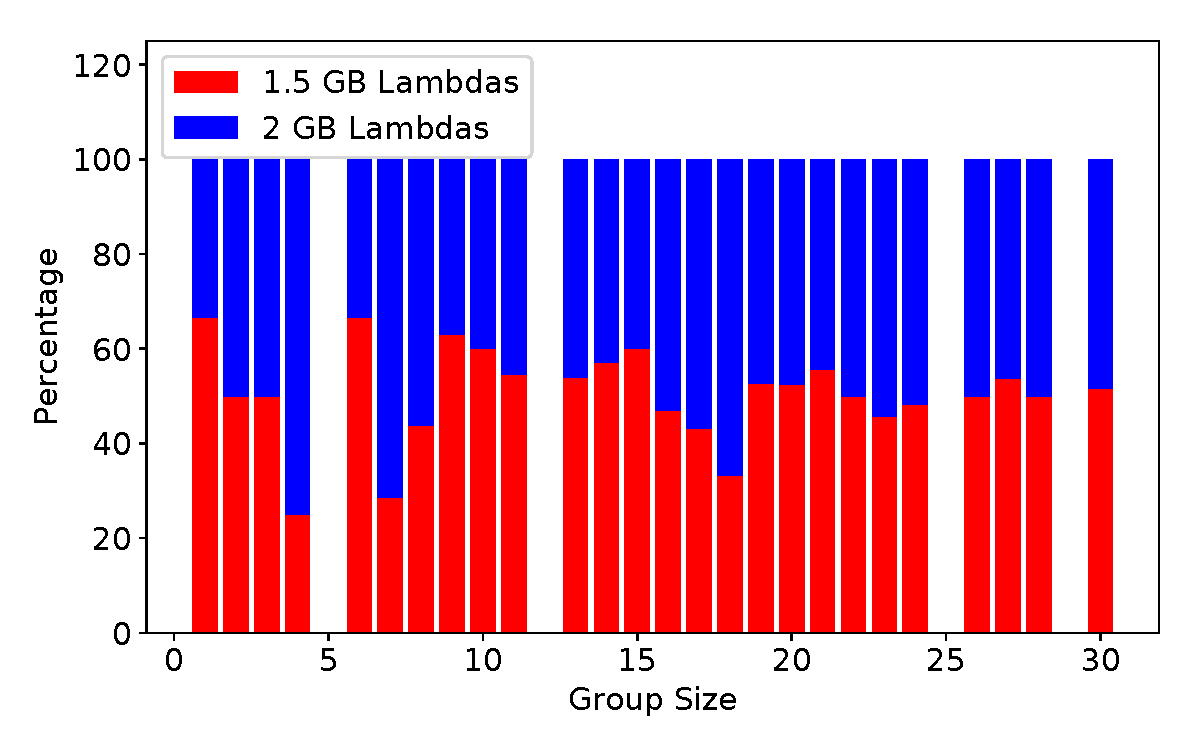
\includegraphics[width=.99\linewidth]{fig/different-sizes.pdf}
    %   \caption{1b}
    %   \label{fig:sfig2}
    \end{subfigure}

    \caption{The left plot shows the breakdown of co-resident groups (of varying
    sizes) of lambdas by two different accounts in an experiment of 1000
    lambdas, where 500 lambdas are launched from each account. The uniformity of
    the split suggests that the lambda scheduler might be invariant to the
    account the lambdas are launched from. Similar results are shown for
    different lambda sizes in the right plot. }
    \label{fig:factors}
\end{figure*}


\subsubsection{Across AWS regions}  
We execute our co-residence detector with 1000 1.5 GB lambdas in various AWS
regions. Figure~\ref{fig:awsregions} comprises multiple plots depicting
the co-resident groups per region, with each bar indicating the fraction of
lambdas that detected a certain number of neighbors (i.e., that belong to a
co-resident group of a certain size). Plots that skew to the right indicate a
higher co-residence density when compared to the plots skewed to the left. 
We note that, in most regions, almost
all lambdas recognize at least one neighbor (indicated by smaller or
non-existent first bar in each plot). We hypothesize that the co-residence
density is (inversely) dependent on the total number of servers and the lambda
activity in the region, both of which can be assumed to be lower in newer AWS
regions resulting in higher co-residence density in those regions. 
Figure~\ref{fig:clusters} shows the total number of co-resident groups with 
two or more lambdas, each of which can be an independent covert channel. 
The ample co-residence in general across all the
regions shows that lambdas provide a fertile ground for covert channels.
%We note that the largest co-resident group on a single machine was comprised of 25 lambdas. 


\subsubsection{Other factors}
We also examine how co-residence is affected by various launch strategies that
the user may use, like deploying lambdas from multiple AWS accounts and
different lambda sizes. In particular, we wish to determine if our mechanism
exhibits different results when: 1) the user deploys sender lambdas and receiver
lambdas on two separate accounts (normally the case with covert channels) and 2)
the senders and receivers are created with different lambdas sizes.  To answer
these questions, we run an experiment with 1000 lambdas of which we launch 500
lambdas from one account (senders) and 500 from the other deployed in a random
order. The co-residence observed was comparable to the case where all the
lambdas were launched from one account. In the left subfigure of
Figure~\ref{fig:factors}, we show the breakdown of co-resident group of lambdas
of each size among the two accounts.  We can see that among the co-resident
groups of all sizes, roughly half of the lambdas came from either account. This suggests 
that lambda scheduler could be agnostic to the accounts the lambdas were launched
from. We see similar results for different lambda sizes, as shown in the right
subfigure of Figure~\ref{fig:factors}.

%From our experiments, we also observe that co-residence density in a region
%barely changes during course of the day or the week (data not shown
%in any figure \todo{is this okay?}).  This gives the user the freedom to utilize this
%technique at any time and expect similar results.

\section{DISCUSSION}
\label{sec:discussion}
\textbf{Alternate use cases}
Our main motivation behind proposing a co-residence detector for lambdas is
to demonstrate the feasibility of a covert channel. However, there are other
scenarios where such tool can be (ab)used, of which we provide a couple of examples. 
\begin{itemize}
%     \item While our co-residence detector does not directly help attackers
%     locate their victims in the cloud, it can aid them in performing devastating 
%     DDOS attacks once by concentrating a number of attack instances on the victim 
%     machine. Also, the attacker could try to gain a wider surface area for 
%     targeted attacks in a cost-effective way by turning on/off her co-resident 
%     instances as necessary. 
    \item Previous studies on performance aspects of lambdas (like performance 
    isolation~\cite{wangusenix2018}) generally need a way to find co-resident
    lambdas. As software-level logical channels begin to disappear, our tool 
    might provide a reliable alternative.
    \item Burst parallel frameworks~\cite{234886} that orchestrate lambdas can
    use our co-residence detector as a locality indicator to take advantage of
    server locality.
\end{itemize}

\noindent \textbf{Mitigation}
In previous section, we showed that our co-residence detector makes the covert
channels practical with lambdas, so it is important that clouds address this
issue. One way to disable our co-residence detector is to fix the underlying
memory bus channel that it employs. However, this only works for newer
generation of servers and is not practical for existing infrastructure. An
easier solution, one that is only practical with lambdas, is to disable the
lambda support for low-level languages (or unsafe versions of high-level
languages) by the cloud providers. This will prevent pointer arithmetic that is
required to activate this channel. However, in all three cloud platforms we examined, 
these unsafe or low level languages were introduced as options at a later point, 
indicating that there is a business use case. In that case, cloud providers may look at
more expensive solutions like BusMonitor~\cite{MemoryBusMitigation} that isolate
memory bus usage for different tenants by trapping the atomic operations to the 
hypervisor. We leave such exploration to future work.

\section{RELATED WORK}
\label{sec:relatedwork}

\textbf{Cloud Attacks} 
Co-residency is possible because of covert channels, so we begin our related
work with an investigation into cloud attacks. Initial
papers in co-residency detection utilized host information and network
addresses arising due to imperfect virtualization~\cite{ristenpartccs2009}.
However, these channels are now obsolete, as cloud provides have
strengthened virtualization and introduced Virtual Private
Clouds~\cite{awsvpc}. Later work used cache-based channels in various levels of
the cache~\cite{xuccsw2011, zhangccs2014, liu2015, kaylaap2016} and hardware
based channels like thermal covert channels~\cite{mastiusenix2015}, RNG
module~\cite{evtyushkinccs2016} and memory bus~\cite{wuusenix2012} have also
been explored in the recent past. Moreover, studies have found that VM
performance can be significantly degraded using memory DDoS
attacks~\cite{zhang2016memory}, while containers are susceptible to power
attacks from adjacent containers~\cite{gao2017}.  

Our work focuses on using the memory bus as a covert channel for determining
cooperative co-residency.  Covert channels using memory bus were first
introduced by Wu et. al~\cite{wuusenix2012}, and subsequently has been used for
co-residency detection on VMs and
containers~\cite{compstudycoresidency,varad191016}  Wu et. al~\cite{wuusenix2012}
introduced a new technique to lock the memory bus by using atomic memory
operations on addresses that fall on multiple cache lines, a technique we rely
on in our own work. \\

\textbf{Co-residency} 
One of the first pieces of literature in detecting VM co-residency was
introduced by Ristenpart et al., who demonstrated that VM co-residency detection
was possible and that these techniques could be used to gather information about
the victim machine (such as keystrokes and network
usage)~\cite{ristenpartccs2009}. This initial work was further expanded in
subsequent years to examine co-residency using memory bus
locking~\cite{xuusenix2015} and active traffic analysis~\cite{bates2012}, as
well as determining placement vulnerabilities in multi-tenant Public
Platform-as-a-Service systems~\cite{varadarajan2015, zhangpaas2016}. Finally,
Zhang et al. demonstrated a technique to detect VM co-residency detection via
side-channel analyses~\cite{zhang2011}. Our work expands on these previous works
by investigating co-residency for lambdas.\\

\textbf{Lambdas} 
While lambdas are a much newer technology than VMs, there still exists lterature
on the subject. Recent studies examined cost comparisons of running web
applications in the cloud on lambdas versus other
architectures~\cite{villamizar2016}, and also examined the lambdas have been
studied in the context of cost-effectivness of batching and data processing with
lambdas~\cite{kiran2015}.  Further research has shown how lambdas perform with
scalability and hardware isolation, indicating some flaws in the lambda
architecture~\cite{wangusenix2018}. From a security perspective, Izhikevich et.
al examined lambda co-residency using RNG and memory bus techniques (similar to
techniques utilized in VM co-residency)~\cite{izhikevich2018}. However, our work
differs from this study in that our technique informs the user of which lambdas
are on the same machine, not only that the lambdas experience co-residency.


\section{ETHICAL CONSIDERATIONS}
As with any large scale measurement project, there are ethical considerations to
take into account. First, there are security and privacy concerns of using this
technique to uncover other consumer's lambdas. However, since we focus on
co-operative co-residence detection, we only determine co-residence for the
lambdas we launched, and do not gain insight into other consumer's lambdas.
Secondly, there is concern that our experiments may cause performance issues
with other lambdas, as we may block their access to the memory bus. We believe
this concern is small, for a number of reasons. Memory accesses are infrequent
due to the multiple levels of caches; we would only be affecting a small number
of operations. Moreover, memory accesses and locking operations are FIFO, which
prevents starvation to the multiple processes sharing a machine. Moreover,
lambdas are generally not recommended for latency-sensitive workloads, due to
their cold-start latencies. Thus, the small amount of lambdas that we might
affect should not, by definition, be affected in their longterm computational
goals. 


\section{CONCLUSION \& FUTURE WORK}
\label{sec:conclusion}
\todo{Copied abstract} 
Cloud computing has seen explosive growth in the past decade. This is made
possible by efficient sharing of infrastructure among tenants, which
unfortunately also raises security challenges like preventing side-channel
attacks. Providers, like AWS and Azure, have traditionally relied on hiding the
co-residency information to prevent targeted attacks in their clouds. But recent
works have repeatedly found co-residence detection techniques that break this
encapsulation, prompting the providers to address them and harden isolation on
their platforms. In this work, we find yet another such technique based on a
memory bus covert channel that is more pervasive, reliable and harder to fix. We
show that we can use this technique to reliably perform co-operative
co-residence detection for thousands of AWS lambdas within a few seconds, which
opens a way for attackers to perform DDoS attacks or learn cloud's internal
mechanisms. We present this technique in detail, evaluate it and use it to
perform a small study on lambda activity across a few AWS regions.  Through this
work, we hope to motivate the need to address this covert channel in the cloud.



\bibliographystyle{ACM-Reference-Format}
\bibliography{paper}

\end{document}
\endinput
%%
%% End of file `sample-sigconf.tex'.
